%%%%%%%%%%%%%%%%%%%%%%%%%%%%% Thesis.tex %%%%%%%%%%%%%%%%%%%%%%%%%%%%%%%
%                                                                      %
%  ---------- Master of Science Dissertation template ----------       %
%                                                                      %
%  Template for the Master Thesis according to the regulations         %
%  published by the Academic Board (Direcção Académica) at IST.        %
%                                                                      %
%  For up-to-date guide, please refer to the official website          %
%  http://academica.tecnico.ulisboa.pt/alunos/dissertacao-de-mestrado/ %
%                                                                      %
%       Andre C. Marta                                                 %
%       Area Cientifica de Mecanica Aplicada e Aeroespacial            %
%       Departamento de Engenharia Mecanica                            %
%       Instituto Superior Tecnico                                     %
%       Av. Rovisco Pais                                               %
%       1049-001 Lisboa                                                %
%       Portugal                                                       %
%       Tel: +351 21 841 9469                                          %
%                        3469 (extension)                              %
%       Email: andre.marta@tecnico.ulisboa.pt                          %
%                                                                      %
%  Created:       Jan 20, 2011                                         %
%  Last Modified: Feb 19, 2018                                         %
%                                                                      %
%%%%%%%%%%%%%%%%%%%%%%%%%%%%%%%%%%%%%%%%%%%%%%%%%%%%%%%%%%%%%%%%%%%%%%%%
%  Revision history                                                    %
%  v1 - 2011/01/24 - original template                                 %
%  v2 - 2012/10/30 - new IST image and glossary support                %
%  v3 - 2013/12/10 - update according to 2012/13 official guide        %
%  v4 - 2014/02/28 - new default for bibliography style                %
%  v5 - 2014/05/07 - update according to 2013/14 official guide        %
%  v6 - 2015/07/02 - cover page format fixed,                          %
%                    contents page numbering fixed,                    %
%                    better language support,                          %
%                    enhanced examples of tables,                      %
%                    new option for appendix page numbering format,    %
%                    custom bibliography style                         %
%  v7 - 2018/02/19 - multiple citations compressed                     %
%%%%%%%%%%%%%%%%%%%%%%%%%%%%%%%%%%%%%%%%%%%%%%%%%%%%%%%%%%%%%%%%%%%%%%%%
%                                                                      %
% To generate the PDF file, type "make" at the terminal prompt.        %
%                                                                      %
% The IST template LaTeX package was created by the author             %
% and it can be downloaded from:                                       %
% https://fenix.ist.utl.pt/homepage/ist31052/                          %
%                                                                      %
% The external packages can be downloaded from                         %
% the Comprehensive TeX Archive Network at http://www.ctan.org/        %
%                                                                      %
% List of LaTex symbols:                                               %
% http://www.ctan.org/tex-archive/info/symbols/comprehensive/          %
%                                                                      %
% Help with LaTex can be found at                                      %
% http://www.giss.nasa.gov/tools/latex/ltx-2.html                      %
% http://en.wikibooks.org/wiki/LaTeX                                   %
%%%%%%%%%%%%%%%%%%%%%%%%%%%%%%%%%%%%%%%%%%%%%%%%%%%%%%%%%%%%%%%%%%%%%%%%

%%%%%%%%%%%%%%%%%%%%%%%%%%%%%%%%%%%%%%%%%%%%%%%%%%%%%%%%%%%%%%%%%%%%%%%%
%     Preamble                                                         %
%%%%%%%%%%%%%%%%%%%%%%%%%%%%%%%%%%%%%%%%%%%%%%%%%%%%%%%%%%%%%%%%%%%%%%%%

% ----------------------------------------------------------------------
%  Set the document class
% ----------------------------------------------------------------------
\documentclass[10pt,a4paper,twoside]{report}

% ----------------------------------------------------------------------
% Define external packages, language, margins, fonts and new commands
% ----------------------------------------------------------------------
%%%%%%%%%%%%%%%%%%%%%%%%%%%%%%%%%%%%%%%%%%%%%%%%%%%%%%%%%%%%%%%%%%%%%%%%
%                                                                      %
%     File: Thesis_Preamble.tex                                        %
%     Tex Master: Thesis.tex                                           %
%                                                                      %
%     Author: Gonçalo Santos                                           %
%     Last modified : 20 Oct 2018                                      %
%                                                                      %
%%%%%%%%%%%%%%%%%%%%%%%%%%%%%%%%%%%%%%%%%%%%%%%%%%%%%%%%%%%%%%%%%%%%%%%%

% ----------------------------------------------------------------------
% Define document language.
% ----------------------------------------------------------------------

% 'inputenc' package
%
% Accept different input encodings.
% http://www.ctan.org/tex-archive/macros/latex/base/
%
% > allows typing non-english text in LaTeX sources.
%
% ******************************* SELECT *******************************
%\usepackage[latin1]{inputenc} % <<<<< Windows
\usepackage[utf8]{inputenc}   % <<<<< Linux
% ******************************* SELECT *******************************


% 'babel' package
%
% Multilingual support for Plain TeX or LaTeX.
% http://www.ctan.org/tex-archive/macros/latex/required/babel/
%
% > sets the variable names according to the language selected
%
% ******************************* SELECT *******************************
%\usepackage[portuguese]{babel} % <<<<< Portuguese
\usepackage[english]{babel} % <<<<< English
% ******************************* SELECT *******************************


% List of LaTeX variable names: \abstractname, \appendixname, \bibname,
%   \chaptername, \contentsname, \listfigurename, \listtablename, ...
% http://www.tex.ac.uk/cgi-bin/texfaq2html?label=fixnam
%
% Changing the words babel uses (uncomment and redefine as necessary...)
%
\newcommand{\acknowledgments}{@undefined} % new LaTeX variable name
%
% > English
%
\addto\captionsenglish{\renewcommand{\acknowledgments}{Acknowledgments}}
%\addto\captionsenglish{\renewcommand{\listtablename}{List of Tables}}
%\addto\captionsenglish{\renewcommand{\listfigurename}{List of Figures}}
%\addto\captionsenglish{\renewcommand{\nomname}{Nomenclature}}
%\addto\captionsenglish{\renewcommand{\appendixname}{Appendix}}
%\addto\captionsenglish{\renewcommand{\bibname}{References}} % Bibliography

% > Portuguese
%
\addto\captionsportuguese{\renewcommand{\acknowledgments}{Agradecimentos}}
%\addto\captionsportuguese{\renewcommand{\listtablename}{Lista de Figuras}}
%\addto\captionsportuguese{\renewcommand{\listfigurename}{Lista de Tabelas}}
\addto\captionsportuguese{\renewcommand{\nomname}{Lista de S\'{i}mbolos}} % Nomenclatura
%\addto\captionsportuguese{\renewcommand{\appendixname}{Anexo}} % Apendice
%\addto\captionsportuguese{\renewcommand{\bibname}{Refer\^{e}ncias}} % Bibliografia


% ----------------------------------------------------------------------
% Define default and cover page fonts.
% ----------------------------------------------------------------------

% Use Arial font as default
%
\renewcommand{\rmdefault}{phv}
\renewcommand{\sfdefault}{phv}

% Define cover page fonts
%
%         encoding     family       series      shape
%  \usefont{T1}     {phv}=helvetica  {b}=bold    {n}=normal
%                   {ptm}=times      {m}=normal  {sl}=slanted
%                                                {it}=italic
% see more examples at
% http://julien.coron.free.fr/languages/latex/fonts/
%
\def\FontLn{% 16 pt normal
  \usefont{T1}{phv}{m}{n}\fontsize{16pt}{16pt}\selectfont}
\def\FontLb{% 16 pt bold
  \usefont{T1}{phv}{b}{n}\fontsize{16pt}{16pt}\selectfont}
\def\FontMn{% 14 pt normal
  \usefont{T1}{phv}{m}{n}\fontsize{14pt}{14pt}\selectfont}
\def\FontMb{% 14 pt bold
  \usefont{T1}{phv}{b}{n}\fontsize{14pt}{14pt}\selectfont}
\def\FontSn{% 12 pt normal
  \usefont{T1}{phv}{m}{n}\fontsize{12pt}{12pt}\selectfont}


% ----------------------------------------------------------------------
% Define page margins and line spacing.
% ----------------------------------------------------------------------

% 'geometry' package
%
% Flexible and complete interface to document dimensions.
% http://www.ctan.org/tex-archive/macros/latex/contrib/geometry/
%
% > set the page margins (2.5cm minimum in every side, as per IST rules)
%
\usepackage{geometry}	
\geometry{verbose,tmargin=2.5cm,bmargin=2.5cm,lmargin=2.5cm,rmargin=2.5cm}

% 'setspace' package
%
% Set space between lines.
% http://www.ctan.org/tex-archive/macros/latex/contrib/setspace/
%
% > allow setting line spacing (line spacing of 1.5, as per IST rules)
%
\usepackage{setspace}
\renewcommand{\baselinestretch}{1.5}


% ----------------------------------------------------------------------
% Include external packages.
% Note that not all of these packages may be available on all system
% installations. If necessary, include the .sty files locally in
% the <jobname>.tex file directory.
% ----------------------------------------------------------------------

% 'graphicx' package
%
% Enhanced support for graphics.
% http://www.ctan.org/tex-archive/macros/latex/required/graphics/
%
% > extends arguments of the \includegraphics command
%
\usepackage{graphicx}


% 'color' package
%
% Colour control for LaTeX documents.
% http://www.ctan.org/tex-archive/macros/latex/required/graphics/
%
% > defines color macros: \color{<color name>}
%
%\usepackage{color}


% 'amsmath' package
%
% Mathematical enhancements for LaTeX.
% http://www.ctan.org/tex-archive/macros/latex/required/amslatex/
%
% > American Mathematical Society plain Tex macros
%
\usepackage{amsmath}  % AMS mathematical facilities for LaTeX.
\usepackage{amsthm}   % Typesetting theorems (AMS style).
\usepackage{amsfonts} %


% 'wrapfig' package
%
% Produces figures which text can flow around.
% http://www.ctan.org/tex-archive/macros/latex/contrib/wrapfig/
%
% > wrap figures/tables in text (i.e., Di Vinci style)
%
% \usepackage{wrapfig}


% 'subfigure' package
%
% Deprecated: Figures divided into subfigures.
% http://www.ctan.org/tex-archive/obsolete/macros/latex/contrib/subfigure/
%
% > subcaptions for subfigures
%
\usepackage{subfigure}


% 'subfigmat' package
%
% Automates layout when using the subfigure package.
% http://www.ctan.org/tex-archive/macros/latex/contrib/subfigmat/
%
% > matrices of similar subfigures
%
\usepackage{subfigmat}


% 'url' package
%
% Verbatim with URL-sensitive line breaks.
% http://www.ctan.org/tex-archive/macros/latex/contrib/url/
%
% > URLs in BibTex
%
% \usepackage{url}


% 'varioref' package
%
% Intelligent page references.
% http://www.ctan.org/tex-archive/macros/latex/required/tools/
%
% > smart page, figure, table and equation referencing
%
%\usepackage{varioref}


% 'dcolumn' package
%
% Align on the decimal point of numbers in tabular columns.
% http://www.ctan.org/tex-archive/macros/latex/required/tools/
%
% > decimal-aligned tabular math columns
%
\usepackage{dcolumn}
\newcolumntype{d}{D{.}{.}{-1}} % column aligned by the point separator '.'
\newcolumntype{e}{D{E}{E}{-1}} % column aligned by the exponent 'E'


% '' package
%
% Reimplementation of and extensions to LaTeX verbatim.
% http://www.ctan.org/tex-archive/macros/latex/required/tools/
%
% > provides the verbatim environment (\begin{verbatim},\end{verbatim})
%   and a comment environment (\begin{comment},  \end{comment})
%
% \usepackage{verbatim}


% 'moreverb' package
%
% Extended verbatim.
% http://www.ctan.org/tex-archive/macros/latex/contrib/moreverb/
%
% > supports tab expansion and line numbering
%
% \usepackage{moreverb}



% 'nomencl' package
%
% Produce lists of symbols as in nomenclature.
% http://www.ctan.org/tex-archive/macros/latex/contrib/nomencl/
%
% The nomencl package makes use of the MakeIndex program
% in order to produce the nomenclature list.
%
% Nomenclature
% 1: On running the file through LATEX, the command \makenomenclature
%    in the preamble instructs it to create/open the nomenclature file
%    <jobname>.nlo corresponding to the LATEX file <jobname>.tex and
%    writes the information from the \nomenclature commands to this file.
% 2: The next step is to invoke MakeIndex in order to produce the
%    <jobname>.nls file. This can be achieved by making use of the
%    command: makeindex <jobname>.nlo -s nomencl.ist -o <jobname>.nls
% 3: The last step is to invoke LATEX on the <jobname>.tex file once
%    more. There, the \printnomenclature in the document will input the
%    <jobname>.nls file and process it according to the given options.
%
% http://www-h.eng.cam.ac.uk/help/tpl/textprocessing/nomencl.pdf
%
% Nomenclature (produces *.nlo *.nls files)
\usepackage{nomencl}
\makenomenclature
%
% Group variables according to their symbol type
%
\RequirePackage{ifthen}
\ifthenelse{\equal{\languagename}{english}}%
    { % English
    \renewcommand{\nomgroup}[1]{%
      \ifthenelse{\equal{#1}{R}}{%
        \item[\textbf{Roman symbols}]}{%
        \ifthenelse{\equal{#1}{G}}{%
          \item[\textbf{Greek symbols}]}{%
          \ifthenelse{\equal{#1}{S}}{%
            \item[\textbf{Subscripts}]}{%
            \ifthenelse{\equal{#1}{T}}{%
              \item[\textbf{Superscripts}]}{}}}}}%
    }{% Portuguese
    \renewcommand{\nomgroup}[1]{%
      \ifthenelse{\equal{#1}{R}}{%
        \item[\textbf{Simbolos romanos}]}{%
        \ifthenelse{\equal{#1}{G}}{%
          \item[\textbf{Simbolos gregos}]}{%
          \ifthenelse{\equal{#1}{S}}{%
            \item[\textbf{Subscritos}]}{%
            \ifthenelse{\equal{#1}{T}}{%
              \item[\textbf{Sobrescritos}]}{}}}}}%
    }%


% 'glossary' package
%
% Create a glossary.
% http://www.ctan.org/tex-archive/macros/latex/contrib/glossary/
%
% Glossary (produces *.glo *.ist files)
\usepackage[number=none]{glossary}
% (remove blank line between groups)
\setglossary{gloskip={}}
% (redefine glossary style file)
%\renewcommand{\istfilename}{myGlossaryStyle.ist}
\makeglossary


% 'rotating' package
%
% Rotation tools, including rotated full-page floats.
% http://www.ctan.org/tex-archive/macros/latex/contrib/rotating/
%
% > show wide figures and tables in landscape format:
%   use \begin{sidewaystable} and \begin{sidewaysfigure}
%   instead of 'table' and 'figure', respectively.
%
\usepackage{rotating}


% 'hyperref' package
%
% Extensive support for hypertext in LaTeX.
% http://www.ctan.org/tex-archive/macros/latex/contrib/hyperref/
%
% > Extends the functionality of all the LATEX cross-referencing
%   commands (including the table of contents, bibliographies etc) to
%   produce \special commands which a driver can turn into hypertext
%   links; Also provides new commands to allow the user to write adhoc
%   hypertext links, including those to external documents and URLs.
%
\usepackage[pdftex]{hyperref} % enhance documents that are to be
                              % output as HTML and PDF
\hypersetup{colorlinks,       % color text of links and anchors,
                              % eliminates borders around links
%            linkcolor=red,    % color for normal internal links
            linkcolor=black,  % color for normal internal links
            anchorcolor=black,% color for anchor text
%            citecolor=green,  % color for bibliographical citations
            citecolor=black,  % color for bibliographical citations
%            filecolor=magenta,% color for URLs which open local files
            filecolor=black,  % color for URLs which open local files
%            menucolor=red,    % color for Acrobat menu items
            menucolor=black,  % color for Acrobat menu items
%            pagecolor=red,    % color for links to other pages
            pagecolor=black,  % color for links to other pages
%            urlcolor=cyan,    % color for linked URLs
            urlcolor=black,   % color for linked URLs
	          bookmarks=true,         % create PDF bookmarks
	          bookmarksopen=false,    % don't expand bookmarks
	          bookmarksnumbered=true, % number bookmarks
	          pdftitle={Thesis},
            pdfauthor={Andre C. Marta},
            pdfsubject={Thesis Title},
            pdfkeywords={Thesis Keywords},
            pdfstartview=FitV,
            pdfdisplaydoctitle=true}


% 'hypcap' package
%
% Adjusting the anchors of captions.
% http://www.ctan.org/tex-archive/macros/latex/contrib/oberdiek/
%
% > fixes the problem with hyperref, that links to floats points
%   below the caption and not at the beginning of the float.
%
\usepackage[figure,table]{hypcap}


% 'natbib' package
%
% Flexible bibliography support.
% http://www.ctan.org/tex-archive/macros/latex/contrib/natbib/
%
% > produce author-year style citations
%
% \citet  and \citep  for textual and parenthetical citations, respectively
% \citet* and \citep* that print the full author list, and not just the abbreviated one
% \citealt is the same as \citet but without parentheses. Similarly, \citealp is \citep without parentheses
% \citeauthor
% \citeyear
% \citeyearpar
%
\usepackage{natbib}


% ----------------------------------------------------------------------
% Define new commands to assure consistent treatment throughout document
% ----------------------------------------------------------------------

\newcommand{\ud}{\mathrm{d}}                % total derivative
\newcommand{\degree}{\ensuremath{^\circ\,}} % degrees

% Abbreviations

\newcommand{\mcol}{\multicolumn}            % table format

\newcommand{\eqnref}[1]{(\ref{#1})}
\newcommand{\class}[1]{\texttt{#1}}
\newcommand{\package}[1]{\texttt{#1}}
\newcommand{\file}[1]{\texttt{#1}}
\newcommand{\BibTeX}{\textsc{Bib}\TeX}

% Typefaces ( example: {\bf Bold text here} )
%
% > pre-defined
%   \bf % bold face
%   \it % italic
%   \tt % typewriter
%
% > newly defined
\newcommand{\tr}[1]{{\ensuremath{\textrm{#1}}}}   % text roman
\newcommand{\tb}[1]{{\ensuremath{\textbf{#1}}}}   % text bold face
\newcommand{\ti}[1]{{\ensuremath{\textit{#1}}}}   % text italic
\newcommand{\mc}[1]{{\ensuremath{\mathcal{#1}}}}  % math calygraphy
\newcommand{\mco}[1]{{\ensuremath{\mathcalold{#1}}}}% math old calygraphy
\newcommand{\mr}[1]{{\ensuremath{\mathrm{#1}}}}   % math roman
\newcommand{\mb}[1]{{\ensuremath{\mathbf{#1}}}}   % math bold face
\newcommand{\bs}[1]{\ensuremath{\boldsymbol{#1}}} % math symbol
\def\bm#1{\mathchoice                             % math bold
  {\mbox{\boldmath$\displaystyle#1$}}%
  {\mbox{\boldmath$#1$}}%
  {\mbox{\boldmath$\scriptstyle#1$}}%
  {\mbox{\boldmath$\scriptscriptstyle#1$}}}
\newcommand{\boldcal}[1]{{\ensuremath{\boldsymbol{\mathcal{#1}}}}}% math bold calygraphy

\usepackage{fancyvrb}
 % file "Thesis_Preamble.tex"

%%%%%%%%%%%%%%%%%%%%%%%%%%%%%%%%%%%%%%%%%%%%%%%%%%%%%%%%%%%%%%%%%%%%%%%%
%     Begin Document                                                   %
%%%%%%%%%%%%%%%%%%%%%%%%%%%%%%%%%%%%%%%%%%%%%%%%%%%%%%%%%%%%%%%%%%%%%%%%
\begin{document}

% Set plain page style (no headers, footer with centered page number)
\pagestyle{plain}

% Set roman numbering (i,ii,...) before the start of chapters
\pagenumbering{roman}

% ----------------------------------------------------------------------
%  Cover page
% ----------------------------------------------------------------------
%%%%%%%%%%%%%%%%%%%%%%%%%%%%%%%%%%%%%%%%%%%%%%%%%%%%%%%%%%%%%%%%%%%%%%%%
%                                                                      %
%     File: Thesis_FrontCover.tex                                      %
%     Tex Master: Thesis.tex                                           %
%                                                                      %
%     Author: Gonçalo Santos                                           %
%     Last modified : 20 Oct 2018                                      %
%                                                                      %
%%%%%%%%%%%%%%%%%%%%%%%%%%%%%%%%%%%%%%%%%%%%%%%%%%%%%%%%%%%%%%%%%%%%%%%%

\thispagestyle {empty}

% IST Logo
% parameters: bb=llx lly urx ury (bounding box), width=h_length, height=v_length, angle=angle, scale=factor, clip=true/false, draft=true/false.
\vspace*{-12mm}
\hspace*{-12mm}

\includegraphics[height=20mm]{IST_A_CMYK_POS-crop.pdf}

\begin{center}
%
% Figure (Image or plot)
\vspace{0.5cm}
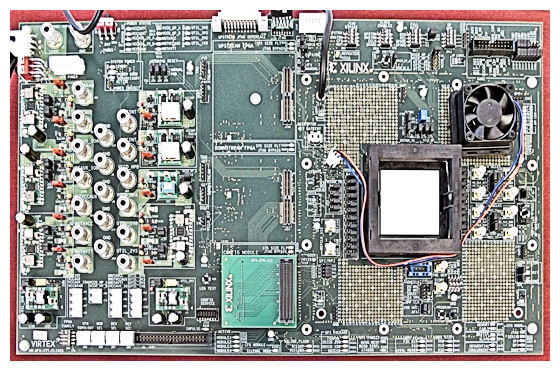
\includegraphics[height=60mm]{Figures/fpga.jpg}

% Title, author and degree
\vspace{0.8cm}
{\FontLb C Compiler for the VERSAT Reconfigurable Processor} \\
\vspace{3.6cm}
{\FontMb Gonçalo da Conceição Reis dos Santos} \\
\vspace{1.9cm}
{\FontLn Thesis to obtain the Master of Science Degree in} \\
\vspace{0.3cm}
{\FontLb Electrical and Computer Engineering} \\
%\vspace{1.9cm}
\vspace{1.0cm}
{\FontSn %
\begin{tabular}{ll}
Supervisor: & Prof. José João Henriques Teixeira de Sousa
\end{tabular} } \\
\vspace{1.0cm}
{\FontMb Examination Committee} \\
\vspace{0.3cm}
{\FontSn %
\begin{tabular}{ll}
Chairperson: & Prof. Francisco André Corrêa Alegria\\
Supervisor: & Prof. José João Henriques Teixeira de Sousa \\
Member of the Committee: & Prof. Paulo Ferreira Godinho Flores \\
\end{tabular} } \\
\vspace{1.5cm}
{\FontMb November 2019} \\
%
\end{center}

\cleardoublepage
 % file "Thesis_FrontCover.tex"
\cleardoublepage

% ----------------------------------------------------------------------
% Dedication page (optional)
% ----------------------------------------------------------------------
%%%%%%%%%%%%%%%%%%%%%%%%%%%%%%%%%%%%%%%%%%%%%%%%%%%%%%%%%%%%%%%%%%%%%%%%%
%                                                                      %
%     File: Thesis_Dedication.tex                                      %
%     Tex Master: Thesis.tex                                           %
%                                                                      %
%     Author: Andre C. Marta                                           %
%     Last modified :  2 Jul 2015                                      %
%                                                                      %
%%%%%%%%%%%%%%%%%%%%%%%%%%%%%%%%%%%%%%%%%%%%%%%%%%%%%%%%%%%%%%%%%%%%%%%%

\null\vskip5cm%
\begin{flushright}
     Dedicated to someone special...
\end{flushright}
\vfill\newpage

 % file "Thesis_Dedication.tex"
%\cleardoublepage

% ----------------------------------------------------------------------
%  Acknowledgments (optional)
% ----------------------------------------------------------------------
%%%%%%%%%%%%%%%%%%%%%%%%%%%%%%%%%%%%%%%%%%%%%%%%%%%%%%%%%%%%%%%%%%%%%%%%%
%                                                                      %
%     File: Thesis_Acknowledgments.tex                                 %
%     Tex Master: Thesis.tex                                           %
%                                                                      %
%     Author: Andre C. Marta                                           %
%     Last modified :  2 Jul 2015                                      %
%                                                                      %
%%%%%%%%%%%%%%%%%%%%%%%%%%%%%%%%%%%%%%%%%%%%%%%%%%%%%%%%%%%%%%%%%%%%%%%%

\section*{\acknowledgments}

% Add entry in the table of contents as section
\addcontentsline{toc}{section}{\acknowledgments}

I want to thank my supervisor, Professor José Teixeira de Sousa, for the 
opportunity to develop this work and for his guidance and support during that process. 
His help was fundamental to overcome the multiple obstacles that I faced during this work.

I also want to acknowledge Professor Horácio Neto for providing a simple Convolutional 
Neural Network application, used as a basis for the application developed for the 
RV32-Versat architecture.

A special acknowledgement goes to my friends, for their continuous support, and Válter,  
that is developing a multi-layer architecture for RV32-Versat. When everything seemed to 
be doomed he always had a miraculous solution.

Finally, I want to express my sincere gratitude to my family for giving me all the 
support and encouragement that I needed throughout my years of study and through the 
process of researching and writing this thesis. They are also part of this work.\\

\textbf{Thank you.}

 % file "Thesis_Acknowledgements.tex"
%\cleardoublepage

% ----------------------------------------------------------------------
%  Abstract (both in English and Portuguese)
% ----------------------------------------------------------------------
%%%%%%%%%%%%%%%%%%%%%%%%%%%%%%%%%%%%%%%%%%%%%%%%%%%%%%%%%%%%%%%%%%%%%%%%%
%                                                                      %
%     File: Thesis_Resumo.tex                                          %
%     Tex Master: Thesis.tex                                           %
%                                                                      %
%     Author: Carlos A. Rodrigues                                           %
%     Last modified : 21 Jan 2011                                      %
%                                                                      %
%%%%%%%%%%%%%%%%%%%%%%%%%%%%%%%%%%%%%%%%%%%%%%%%%%%%%%%%%%%%%%%%%%%%%%%%

\section*{Resumo}

% Add entry in the table of contents as section
\addcontentsline{toc}{section}{Resumo}

Inserir o resumo em Portugu\^{e}s aqui com o máximo de 250 palavras e acompanhado de 4 a 6 palavras-chave...

\vfill

\textbf{\Large Palavras-chave:} OpenRISC, Sistema em um chip,...

\cleardoublepage

   % file "Thesis_Resumo.tex"
%\cleardoublepage

%%%%%%%%%%%%%%%%%%%%%%%%%%%%%%%%%%%%%%%%%%%%%%%%%%%%%%%%%%%%%%%%%%%%%%%%%
%                                                                      %
%     File: Thesis_Abstract.tex                                        %
%     Tex Master: Thesis.tex                                           %
%                                                                      %
%     Author: Andre C. Marta                                           %
%     Last modified :  2 Jul 2015                                      %
%                                                                      %
%%%%%%%%%%%%%%%%%%%%%%%%%%%%%%%%%%%%%%%%%%%%%%%%%%%%%%%%%%%%%%%%%%%%%%%%

\section*{Abstract}

% Add entry in the table of contents as section
\addcontentsline{toc}{section}{Abstract}

Versat is a Coarse-Grain Reconfigurable Array architecture (CGRA), which
implements self and partial reconfiguration by using a simple controller
unit. This report studies the current state of the art in HDL and CGRA
simulation, providing a basis to the development of a simulation environment for
Versat. The main objective of this environment is to provide a faster way to
develop and debug software without the use of prototyping hardware. Therefore,
the two types of HDL simulators, event-driven and cycle-accurate, their
advantages and disadvantages are studied, along with a performance comparison
between them. A study of high-level implementations for CGRA simulation is
also presented.

\vfill

\textbf{\Large Keywords:} Versat, coarse-grain reconfigurable arrays, HDL
simulation, CGRA simulation, high-level simulation

 % file "Thesis_Abstract.tex"
%\cleardoublepage

% ----------------------------------------------------------------------
%  Table of contents, list of tables, list of figures and nomenclature
% ----------------------------------------------------------------------

% Table of contents
%
\tableofcontents
\cleardoublepage 

% List of tables
%
% Add entry in the table of contents as section
%\phantomsection
%\addcontentsline{toc}{section}{\listtablename}
% Generate list
%\listoftables
%\cleardoublepage 

% List of figures
%
% Add entry in the table of contents as section
%\phantomsection
%\addcontentsline{toc}{section}{\listfigurename}
% Generate list
%\listoffigures
%\cleardoublepage 

% Nomenclature
%
% entries of nomenclature list
%%%%%%%%%%%%%%%%%%%%%%%%%%%%%%%%%%%%%%%%%%%%%%%%%%%%%%%%%%%%%%%%%%%%%%%%%
%                                                                      %
%     File: Thesis_Nomenclature.tex                                    %
%     Tex Master: Thesis.tex                                           %
%                                                                      %
%     Author: Gonçalo Santos                                           %
%     Last modified : 20 Oct 2018                                      %
%                                                                      %
%%%%%%%%%%%%%%%%%%%%%%%%%%%%%%%%%%%%%%%%%%%%%%%%%%%%%%%%%%%%%%%%%%%%%%%%
%
% The definitions can be placed anywhere in the document body
% and their order is sorted by <symbol> automatically when
% calling makeindex in the makefile
%
% The \glossary command has the following syntax:
%
% \glossary{entry}
%
% The \nomenclature command has the following syntax:
%
% \nomenclature[<prefix>]{<symbol>}{<description>}
%
% where <prefix> is used for fine tuning the sort order,
% <symbol> is the symbol to be described, and <description> is
% the actual description.

% ----------------------------------------------------------------------
% Roman symbols [r]
\nomenclature[ru]{$\bf u$}{Velocity vector.}
\nomenclature[ru]{$u,v,w$}{Velocity Cartesian components.}
\nomenclature[rp]{$p$}{Pressure.}
\nomenclature[rC]{$C_D$}{Coefficient of drag.}
\nomenclature[rC]{$C_L$}{Coefficient of lift.}
\nomenclature[rC]{$C_M$}{Coefficient of moment.}

% ----------------------------------------------------------------------
% Greek symbols [g]
\nomenclature[g]{$\rho$}{Density.}
\nomenclature[g]{$\alpha$}{Angle of attack.}
\nomenclature[g]{$\beta$}{Angle of side-slip.}
\nomenclature[g]{$\mu$}{Molecular viscosity coefficient.}
\nomenclature[g]{$\kappa$}{Thermal conductivity coefficient.}

% ----------------------------------------------------------------------
% Subscripts [s]
\nomenclature[s]{$x,y,z$}{Cartesian components.}
\nomenclature[s]{$i,j,k$}{Computational indexes.}
\nomenclature[s]{$\infty$}{Free-stream condition.}
\nomenclature[s]{ref}{Reference condition.}
\nomenclature[s]{$n$}{Normal component.}

% ----------------------------------------------------------------------
% Supercripts [t]
\nomenclature[t]{T}{Transpose.}
\nomenclature[t]{*}{Adjoint.}

 % file "Thesis_Nomenclature.tex"
%
% Add entry in the table of contents as section
%\phantomsection
%\addcontentsline{toc}{section}{\nomname}
% Insert glossary/nomenclature section produced by MakeIndex
%\printnomenclature
%\cleardoublepage

% entries of glossary list
%%%%%%%%%%%%%%%%%%%%%%%%%%%%%%%%%%%%%%%%%%%%%%%%%%%%%%%%%%%%%%%%%%%%%%%%%
%                                                                      %
%     File: Thesis_Glossary.tex                                        %
%     Tex Master: Thesis.tex                                           %
%                                                                      %
%     Author: Carlos A. Rodrigues                                           %
%     Last modified : 30 Oct 2012                                      %
%                                                                      %
%%%%%%%%%%%%%%%%%%%%%%%%%%%%%%%%%%%%%%%%%%%%%%%%%%%%%%%%%%%%%%%%%%%%%%%%
%
% The definitions can be placed anywhere in the document body
% and their order is sorted by <symbol> automatically when
% calling makeindex in the makefile
%
% The \glossary command has the following syntax:
%
% \glossary{entry}
%
% The \nomenclature command has the following syntax:
%
% \nomenclature[<prefix>]{<symbol>}{<description>}
%
% where <prefix> is used for fine tuning the sort order,
% <symbol> is the symbol to be described, and <description> is
% the actual description.

% ----------------------------------------------------------------------

\glossary{name={\textbf{MDO}},description={Multi-Disciplinar Optimization is an engineering technique that uses optimization methods to solve design problems incorporating two or more disciplines.}}

\glossary{name={\textbf{CFD}},description={Computational Fluid Dynamics is a branch of fluid mechanics that uses numerical methods and algorithms to solve problems that involve fluid flows.}}

\glossary{name={\textbf{CSM}},description={Computational Structural Mechanics is a branch of structure mechanics that uses numerical methods and algorithms to perform the analysis of structures and its components.}}

 % file "Thesis_Glossary.tex"

% Add entry in the table of contents as section
%\phantomsection
%\addcontentsline{toc}{section}{\glossaryname}
% Insert glossary section produced by MakeIndex
%\printglossary
%\cleardoublepage

% Set arabic numbering (1,2,...) after preface
%
\setcounter{page}{1}
\pagenumbering{arabic}

% ----------------------------------------------------------------------
%  Chapters
% ----------------------------------------------------------------------

%%%%%%%%%%%%%%%%%%%%%%%%%%%%%%%%%%%%%%%%%%%%%%%%%%%%%%%%%%%%%%%%%%%%%%%%
%                                                                      %
%     File: Thesis_Introduction.tex                                    %
%     Tex Master: Thesis.tex                                           %
%                                                                      %
%     Author: Andre C. Marta                                           %
%     Last modified :  2 Jul 2015                                      %
%                                                                      %
%%%%%%%%%%%%%%%%%%%%%%%%%%%%%%%%%%%%%%%%%%%%%%%%%%%%%%%%%%%%%%%%%%%%%%%%

\chapter{Introduction}
\label{chapter:introduction}




In this report, the problem of accelerating the execution of Deep Neural
Networks (DNNs) using Coarse GRained Reconfigurable Arrays (CGRAs) is studied,
with special emphasis on compiling a DNN description into code that runs on
CPU/CGRA system. The Deep Versat Architecture~\cite{valter:deepversat} CGRA will be used as an
implementation tool in this work.


%%%%%%%%%%%%%%%%%%%%%%%%%%%%%%%%%%%%%%%%%%%%%%%%%%%%%%%%%%%%%%%%%%%%%%%%
\section{Problem}
\label{section:problem}

Neural Networks have been an object of study since the 1940's, but until the
beginning of this decade their applications were limited and did not play a
major role in computer vision conferences. With its meteoric rise in research,
several solutions to accelerate this algorithm have appeared, from Field Programmable Gate Arrays (FPGA) to
Application Specific Integrated Circuits (ASIC) implementations.

Convolutional Neural Networks (CNNs) are a particular kind of DNN where the output
values of the neurons in one layer are convolved with a kernel to produce the
input values of the neurons of the next layer. This algorithm is compute bound,
that is, its performance depends on how fast it can do certain calculations, and
depend less on the memory access time. Namely the convolutional layers take
approximately 90$\%$ of the computation time.

The acceleration of these workloads is a matter of importance for today's
applications such as image processing for object recognition or simply to
enhance certain images. Other uses like instant translation and virtual
assistants are applications of neural networks and their acceleration is of
vital importance to bring them into Internet of Things.

A suitable circuit to accelerate DNNs in hardware is the CGRA. A CGRA is a
collection of Functional Units and memories with programmable interconnections
in order to form computational datapaths. A CGRA can be implemented in both
FPGAs and ASICs. CGRAs can be reconfigured much faster than FPGAs, as they have
much less configuration bits. If reconfiguration is done at runtime, CGRAs add
temporal scalability to the spacial scalability that characterize
FPGAs. Moreover, partial reconfiguration is much easier to do in CGRAs compared
to FPGAs which further speeds up reconfiguration time. Another advantage of
CGRAs is the fact that they can be programmed entirely in software, contrasting
with the large development time of customized Intellectual Property (IP) blocks.
The Coarse Grain Reconfigurable Arrays (CGRA) is a midway acceleration solution
between FPGAs, which are flexible but large, power hungry and difficult to
reprogram, and ASICs, which are fast but generally not programmable.

However, mapping a specific DNN to a CGRA requires knowledge of its
architecture, latencies and register configurations, which may become a lengthy
process, especially if the user wants to explore the design space for several
DNN configurations. An automatic compiler that can map a standard DNN
description into CPU/CGRA code would dramatically decrease time to market of its
users. Currently there are equivalent tools for CPUs and GPUs and
even for FPGAS.


%%%%%%%%%%%%%%%%%%%%%%%%%%%%%%%%%%%%%%%%%%%%%%%%%%%%%%%%%%%%%%%%%%%%%%%%
\section{Solution}
\label{section:solution}

The proposed solution is a compiler that takes a configuration file from a
neural network framework like Caffe or Darknet. This new tool inputs the
parameters of Deep Versat, such as the number of layers and functional units,
and produces the C code needed for the Versat runs. This code is run on the
RISC-V picorv32~\cite{picorv} CPU controller that has Deep Versat as a peripheral.

%%%%%%%%%%%%%%%%%%%%%%%%%%%%%%%%%%%%%%%%%%%%%%%%%%%%%%%%%%%%%%%%%%%%%%%%
%\section{Thesis Outline}
%\label{section:outline}

%Briefly explain the contents of the different chapters...

%%%%%%%%%%%%%%%%%%%%%%%%%%%%%%%%%%%%%%%%%%%%%%%%%
%\section{Author's Work}
%\label{section:authorwork}

%TO ADD----

%%%%%%%%%%%%%%%%%%%%%%%%%%%%%%%%%%%%%%%%%%%%%%%%%%
\section{Report Outline}
\label{reportoutline}

This report is composed of 4 more chapters. In the second chapter, the
state-of-the-art of neural networks and the difficulties accelerating them is
described. In the third chapter, the Deep Versat architecture and how to program
it is explained. In the fourth chapter, CNN compiler techniques are
explored. Finally, the last chapter contains the proposed solution and the plan
for its execution.


 % file "Thesis_Introduction.tex"
%\cleardoublepage

\chapter{CNN Background}
\label{chapter:background}

%This chapter is the main one for the IIEEC report, it contains the section about \textbf{Framing of the thesis theme in the scientific area and state of the art revision}.
%%%%%%%%%%%%%%%%%%%%%%%%%%%%%%%%%%%%%%%%%%%%%%%%%%%%%%%%%%%%%%%%%%%%%%%%%
%
%Things I need to talk about:
%\begin{itemize}
%    \item What are neural networks being used for - general introduction
%    \item architecture of neural networks: more terminology: input, output, hidden layers...
%    \item Training vs Inference
%    \item Basic neural network operations: weights, biases, Activations (Fully Connected Layer)
%    \item Deep neural networks: advantages, difficulties
%    \item Convolutional Neural Networks (CNN): basic operation, some intuition, results (e.g ImageNet)
%    \item 3 basic ideias of CNNs: local receptive fields, shared weights, pooling
%    \item introduce terminology: kernel/filter, feature map
%    \item putting all factors that make DNNs, more specifically CNNs work
%    \item factors for effective training (and problems)
%\end{itemize}{}
%
%\newpage

Convolutional neural networks (CNNs) were introduced in 1989 by Yann LeCun for
digit recognition~\cite{lecun:handwritten_zipcodes89}. Since then CNNs have
increased in size and complexity and have gained popularity in the last years
for applications like speech processing, robotics and image processing. One
example is the performance of AlexNet~\cite{AlexNetKrizhevsky:2012} at the
ImageNet Large Scale Visual Recognition Challenge
2012~\cite{ImageNet2012_ILSVRC15}.

In this chapter a background for CNNs is established. The first sections
introduce the concepts of inference and training of neural networks. Then, the
main types of layers found in CNNs are presented. In the final part of the
chapter, an analysis of the YOLOv3~\cite{yolov3} network, a CNN used for image
detection, is presented.


%Since the result of the AlexNet \cite{AlexNetKrizhevsky:2012} at the ImageNet Large Scale Visual Recognition Challenge 2012 \cite{ImageNet2012_ILSVRC15}, convolutional neural networks have been used for image recognition applications.

\section{Neural Networks}
\label{section:neural_networks}

% Neural networks have gained popularity in the last years due to accuracy on applications like speech processing, robotics and image processing.
\begin{figure}[!htb]
	\centering
	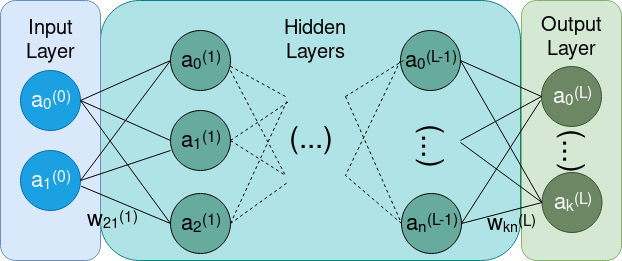
\includegraphics[width=0.70\textwidth]{Figures/FCNN.png}
	\caption[Caption for figure in TOC.]{Neural Network Structure}
	\label{fig:FCNN}
\end{figure}

The most basic element of neural networks is the neuron. The output value $a$ of
a neuron is given by
\begin{equation}
a  = \sigma\Big( b + \sum_{i=0}^{n-1} w_{i}\times x_i \Big),
\label{eq:neuron_value}
\end{equation}
where $w_i$ is the weight associated with input $x_i$, $b$ is a parameter called
bias, $\sigma(.)$ is called the activation function and $n$ is the number of
inputs of the neuron.

Fig.~\ref{fig:FCNN} presents a neural network. Neurons are organized in layers
where the neurons in one layer only receive input values from the same set of
previous layers. If the input values are the neural network inputs, the layer is
called the \underline{input layer}. The values calculated at the input layer
neurons are sent to the next layer. The last layer of the network is called the
\underline{output layer}. The layers in between are called \underline{hidden
  layers}.

Activations are non-linear functions applied to each neuron output. The non-linearity
of the activation functions allows for multiple layer networks to approximate
any function~\cite{mnielsen:nnanddl}. The sigmoid function, presented in
Fig.~\ref{fig:sigmoid}, is one of the first functions used. In the last years,
the Rectified Linear Unit (ReLU), Fig.~\ref{fig:ReLU}, and some variations like
the leaky ReLU, Fig.~\ref{fig:leaky}, have gained popularity due to the reduced
computational complexity during network training.
%\begin{equation}
%\begin{cases}
%Sigmoid(x) = \frac{1}{1 + \exp(-x)} \\
%ReLU(x) = max\{0, x \}\\
%Leaky_{ReLU}(x) = max\{0.1x, x\}
%\label{eq:activation_functions}
%\end{cases}
%\end{equation}

\begin{figure}[!htb]
	\begin{subfigmatrix}{3}
		\subfigure[Sigmoid Activation]{\label{fig:sigmoid} 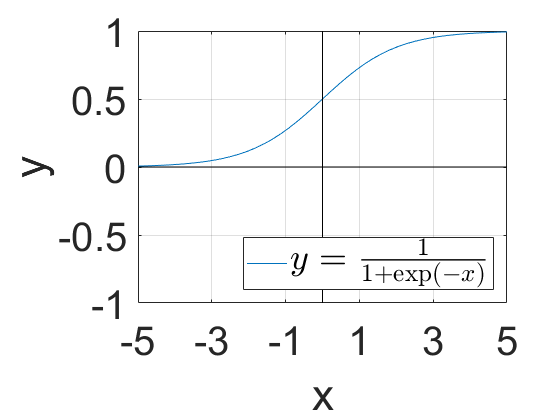
\includegraphics[width=0.32\textwidth]{Figures/sigmoid.png}}
		\subfigure[ReLU Activation]{\label{fig:ReLU} 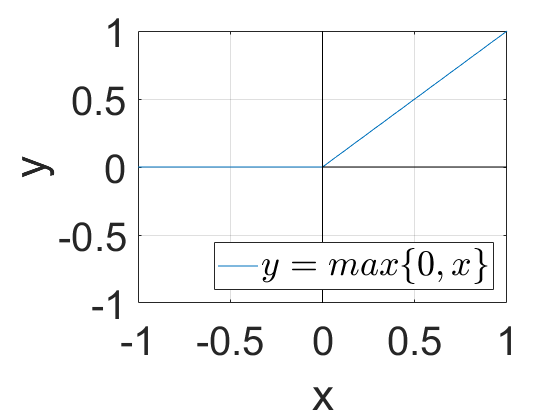
\includegraphics[width=0.32\textwidth]{Figures/ReLU.png}}
		\subfigure[Leaky ReLU Activation]{\label{fig:leaky} 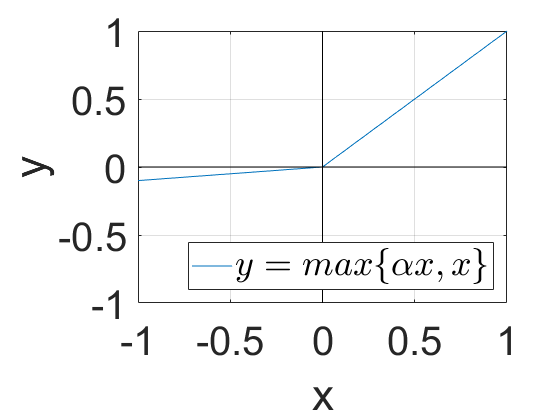
\includegraphics[width=0.32\textwidth]{Figures/leaky_ReLU.png}}		
	\end{subfigmatrix}
	\caption{Plots of common activation functions}
	\label{fig:activation_plots}
\end{figure}

\section{Neural Network Inference}
\label{section:inference}
Inference corresponds to the operation of the network over data outside of the
training dataset using the already trained weights and biases. The key idea
behind this mode is that if the input data being received is similar to the data
used for training, then the output generated by the network should reach a
comparable accuracy with the one achieved during training.

\section{Neural Network Training}
\label{section:training}
Neural networks are trained using a training dataset that contains inputs for
the network and the desired outputs. During training, the weights and biases of
the network are tuned so that given the dataset inputs, the output generated is
as close as possible to the desired output. Training is based on gradient
descent techniques that update the weights and biases of the network based on
the partial derivatives of each value with respect to the difference between the
desired output and the one generated by the network. The backpropagation
algorithm is the main method used for network training. Training is demanding in
terms of computation and memory. The training process is often done in a
separate machine, usually taking advantage of the computation capabilities of
GPUs.

\section{Fully-Connected Network}
\label{subsection:fc_network}

In fully-connected layers, each neuron receives the outputs from all neurons of
the previous layer, where there is a different weight associated for each input
value. In fact, Fig.~\ref{fig:FCNN} depicts a neural network composed
exclusively by fully-connected layers.


%In general the fully-connected layers appear at the end of the network to perform the classification of the features detected by the convolutional layers.

%intro to deep neural networks into CNNs
% 3 basic ideias - introduce terminology
% talk about convolution - pooling - normalization - activations
% quantitative factors to CNNs (throughout the previous text?)

%\subsection{Deep Neural Networks (DNNs)}
%\label{subsection:dnns}
%For the application of image processing, the intuition of how the network works is related with each neuron being able to detect one pattern. With more layers, the neurons on the first layers detect simple patterns that are progressively compounded into more complex patterns across the layers, up to the output layer, where the object detection is done. Following this logic, it is expected that deep neural networks can be more powerful than a shallow network. However, this comes with additional difficulties in training all the weights and biases for networks of increasing depth. This problem is usually circumvented by replacing the fullyconnected layers with convolutional layers.

\section{Convolutional Neural Networks (CNNs)}
\label{section:cnns}

Unlike fully-connected networks, CNNs are mainly composed by convolutional
layers. Other commonly found layers in CNNs are pooling, batch normalization,
routing, upsample and shortcut layers.

% Convolutional neural networks are based on three basic ideas: \underline{local receptive fields}, \underline{shared weights} and \underline{pooling} \cite{mnielsen:nnanddl}.


\subsection{Convolutional Layer}
\label{subsection:conv_layer}

In convolutional layers, a neuron only depends on a small number of inputs,
which corresponds to the neuron only analysing a specific feature for a region
of the input. The specific region is called local receptive
  field. Hence, associated with each neuron, there is only a reduced number of
weights and one bias.

In fact, the same local weights and bias are used for a set of neurons, which
corresponds to searching for the same feature in the entire input, making
convolution invariable to translation in images. The shared weights form a
\underline{kernel}.

%This process creates a \underline{feature map (FM)} of the input, due to using the same \underline{shared weights} and \underline{shared bias} over a small region that is overlapped onto an image like a sliding window. 
% and for each layer multiple kernels can be used to generate multiple corresponding feature maps.

The input of convolutional layers is divided into $C$ channels, where each
channel is defined as a ($W\times H$) \underline{feature map (FM)}. For example,
in Fig.~\ref{fig:3D_conv} the input has 3 channels and each feature map has size
$6\times 6$.

Each kernel used in the convolution has $C$ channels, the same as the input. The
number of output channels is the same as the number of kernels used. Each value
on the output is the accumulation of the products of the input with the
overlapped kernel.

\begin{figure}[!htb]
	\centering
	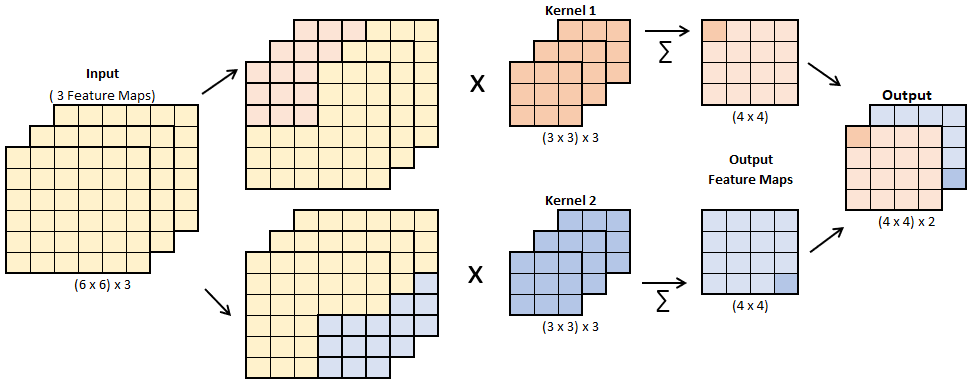
\includegraphics[width=0.70\textwidth]{Figures/3D_convolution.png}
	\caption[Caption for figure in TOC.]{Example of a 3D convolution}
	\label{fig:3D_conv}
\end{figure}

%Fig. \ref{fig:3D_conv} presents an example of a 3D convolution. Given an input composed of multiple feature maps (channels), multiple three dimensional kernels with the same number of channels are used for convolution, creating one output feature map per kernel. The number of output channels is the same as the number of kernels used. Each value on the output is the accumulation of the products of the input with the overlapped kernel.

\subsection{Pooling Layer}
\label{subsection:pool_layer}
CNNs commonly use \underline{pooling} layers to reduce the size of the feature
maps. Intuitively this corresponds to only keeping a rough idea of the feature
location. The reduction of the feature maps also reduces the amount of
computation at latter layers of the network. The most common pooling operations
divide the feature map into $2\times2$ regions and select either the larger
(Max-pooling) or the average (Average-pooling) value.

% figure of max pooling?

\subsection{Batch Normalization Layer}
\label{subsection:batch_norm_layer}
Batch normalization sets the average of the input values to zero and the
standard variation to one. After that, the values are scaled and shifted using
the ($\gamma$,$\beta$) parameters also learned in training. This control of the
input distribution speeds up training and improves
accuracy~\cite{sze:dnn_tutorial}. For a given value $x$, the normalization
outputs

%As the depth of the network increases, the input value distribution across
%layers is a factor that can impact the speed of training. That problem is
%reduced with batch normalization that sets the average to zero and the standard
%variation to one and then the value is scaled and shifted using the
%($\gamma$,$\beta$) parameters also learned in training. For a given value $x$,
%the normalization outputs

\begin{equation}
y = \frac{x - \mu}{\sqrt{\sigma^2 + \epsilon}}\gamma + \beta
\label{eq:batch_normalization}
\end{equation}
Since all variables are known after training, is possible to rewrite (\ref{eq:batch_normalization}) as 
\begin{equation}
\frac{\gamma}{\sqrt{\sigma^2 + \epsilon}}x + \Bigg(-\frac{\mu}{\sqrt{\sigma^2 + \epsilon}}\gamma + \beta  \Bigg) = Ax + B,
\label{eq:batch_normalization_macc}
\end{equation}
which avoids the computation of the square root and division.  The additional
$\epsilon$ term is used to avoid numerical errors related with denominators too
close to zero.

\subsection{Routing Layer}
\label{subsection:route_layer}
Routing layers are used to get an output from a previous layer in the network. If multiple previous layers are selected, their output is concatenated.

\subsection{Upsample Layer}
\label{subsection:upsample_layer}
Upsample layers increase the size of the input FMs, doubling their width and
height. The simplest upsample method consists in repeating each value in a FM
four times in a $2\times 2$ square.

\subsection{Shortcut Layer}
\label{subsection:shortcut_layer}
Shortcut layers add the output from two or more previous layers in the network
pipeline. Shortcut layers are used to mitigate the vanishing gradient problem
that arises during training for networks with considerable depth. With this
addition, the networks act as already knowing the result from the further back
layer and only need to learn a residual to get the desired outcome. Shortcut
layers are common on ResNet
networks~\cite{ResNet_2015DBLP:journals/corr/HeZRS15}.

\section{YOLO}
YOLO (You Only Look
Once)~\cite{Yolov1_DBLP:journals/corr/RedmonDGF15,Yolov2_redmon2016yolo9000,yolov3}
is an object detection and classification system that is composed of a single
CNN that receives an image and outputs bounding box coordinates and class
probabilities from the detected objects.

A YOLO network is composed of a sequence of convolutional layers that serve as
feature extractors at different scales. During these layers of the network, the
size of the FMs is gradually reduced whether by pooling layers or convolutional
layers with stride 2, depending on the network version.

After the feature extraction, object detection and classification is done at
different FM sizes, which corresponds to analysing the input image at different
$g_i \times g_i$ grids.

For each cell in each grid, $M$ attempts of object detection are done. Each
attempt is represented by \underline{two} values for the \underline{object box
  center}, \underline{two} for the \underline{object box size}, \underline{one}
value for the \underline{objectness score} and \underline{80 class scores}. The
objectness score indicates the likelihood of the detection corresponding to an
object. The 80 class scores correspond to the number of existing classes in the
COCO dataset~\cite{coco:Microsoft} used for training. In total an object
detection attempt is represented by $(2+2+1+80) = 85$ values.

Before the object detection and classification at grid size $g_i \times g_i$
starts, a set of $(M \times 85)$ FMs of size $ g_i \times g_i$ is created, and
each detection value is associated with a specific FM.

%In total there are $ M \times (1+2+2+80) = M\times 85$ values per grid cell,
%which corresponds to the $M\times 85$ FMs at the input of the yolo layers. The
%size of each FM at the yolo layer input corresponds to the grid size used for
%the detection.


%Each attempt is represented by one value for the objectness score, which
%indicates the likelihood of the detection corresponding to an object; two
%values for the object box position and two for the object box size; and 80
%scores, one for each class being classified. In total there are $ 3 \times
%(1+2+2+80) = 255$ values per grid cell, which corresponds to the $255$ FMs at
%the input of the yolo layers. The size of each FM at the yolo layer input
%corresponds to the grid size.

The object detection and classification process uses a custom type of layer
called \underline{yolo layer}. At the yolo layers, the FMs of the channels
corresponding to the \underline{box coordinates}, \underline{objectness score}
and \underline{classes scores} are passed through a sigmoid activation function
(Fig.~\ref{fig:sigmoid}). The channels for each output type and the activation
performed at the yolo layer is presented in
Tab.~\ref{tab:yolov3_channel_division}, for the case of $M=3$. The outputs of
the several yolo layers correspond to the outputs of the network.

\begin{table}[!htb]
	\renewcommand{\arraystretch}{1.2} % more space between rows
	\centering
	\begin{tabular}{ccc}
		\toprule
		Channel Ranges           & Outputs & Activation  \\
		\midrule
		$\{[0,1];[85,86];[170,171]\}$       & Box center coordinates   & Sigmoid \\
		$\{[2,3];[87,88];[172,173]\}$       & Box size   & None \\
		$\{4;89;174\}$       & Objectness score   & Sigmoid \\
		$\{[5-84];[90-169];[175-254]\}$       & Class scores   & Sigmoid \\
		\bottomrule
	\end{tabular}
	\caption[Table caption shown in TOC.]{Yolo layer channel composition and performed activations for $M=3$.}
	\label{tab:yolov3_channel_division}
\end{table}

After all the outputs of the network are obtained, all the detections done by
the network need to be filtered. This consists in excluding detections with an
objectness score below a determined threshold; and then applying Non-maximum
Suppression (NMS) to eliminate multiple detections of the same object. The NMS
process starts from the detection with highest objectness score and resorts to a
Intersection over Union (IoU), illustrated in Fig.~\ref{fig:IoU}, 
between the current detection box and all the
others. If the result is above the IoU
threshold, the detection with the lowest objectness score is discarded,
otherwise it is kept. This is done for all remaining detections in a descending
order of objectness score.
\begin{figure}[!htb]
	\centering
	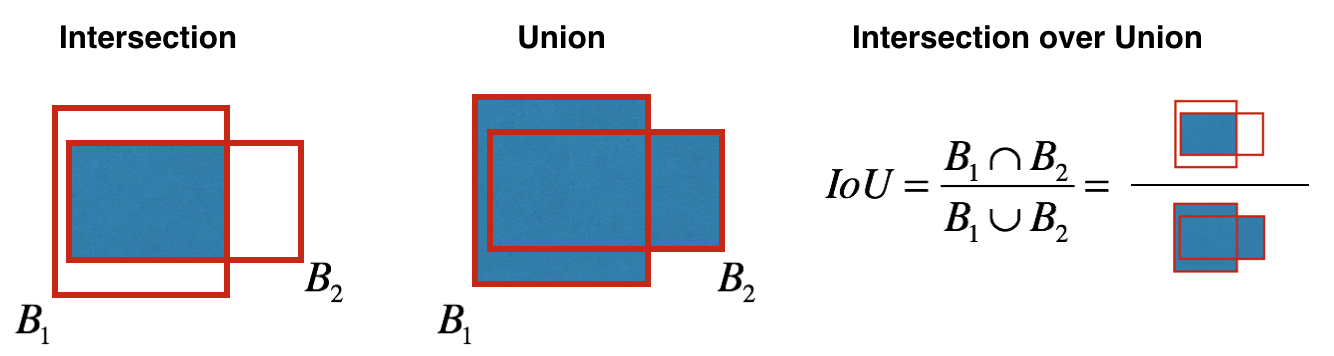
\includegraphics[width=0.5\textwidth]{Figures/IoU.png}
	\caption[Caption for figure in TOC.]{Diagram of the Intersection over Union (IoU) calculation, from~\cite{IoU_image_credit}}
	\label{fig:IoU}
\end{figure}

\subsection{Accuracy Metrics}
\label{sec:map}


The mean Average Precision (mAP) is a measure used to compare networks that use the Common Objects in
Context (COCO) dataset~\cite{coco:Microsoft}.

%FIX explanation
%The mAP metric gives an indication of the degree to which the correct
%classification have the highest confidence levels.
%???(FIXED) - isto não esta aqui a fazer nada, mas vale nao confundir


The mAP is the average of the
AP calculated for each class. The AP is calculated by ordering the
classifications performed by the highest bounding box confidence level. The
classifications are evaluated as true positives or false positives according to the ground truth. At each classification is also calculated the precision and recall, given by
\begin{equation}
	recall = \frac{\#True \ Positives}{\# Total True Positives} \text{ and } precision = \frac{\# True \ Positives}{\# Classifications}.
	\label{eq:precision_recall}
\end{equation}
The true positives are the number of correct classifications up to the classification being analysed and the total true positives are the total number of objects in the image. The number of classifications corresponds to the order of the classification being analysed. A precision/recall curve is calculated with the values computed for each classification as is presented by the orange curve in Fig.~\ref{fig:mAP}. The curve is then altered in order to have monotonically decreasing precision, by setting the precision at a given point equal to the maximum precision for any value of higher recall, as is presented by the green curve in Fig.~\ref{fig:mAP}. Finally, the AP is calculated by computing the area under the green curve.
%The mAP is the average of the
%AP calculated for each class. The AP is calculated by ordering the
%classifications performed by the highest bounding box confidence level. The
%classifications are evaluated as true positives or false positives according to the ground truth. From each
%true positive found onwards, the classifications receive the score of the recall
%at the true positive.
% how to decide if true or false?
\begin{figure}[!htb]
	\centering
	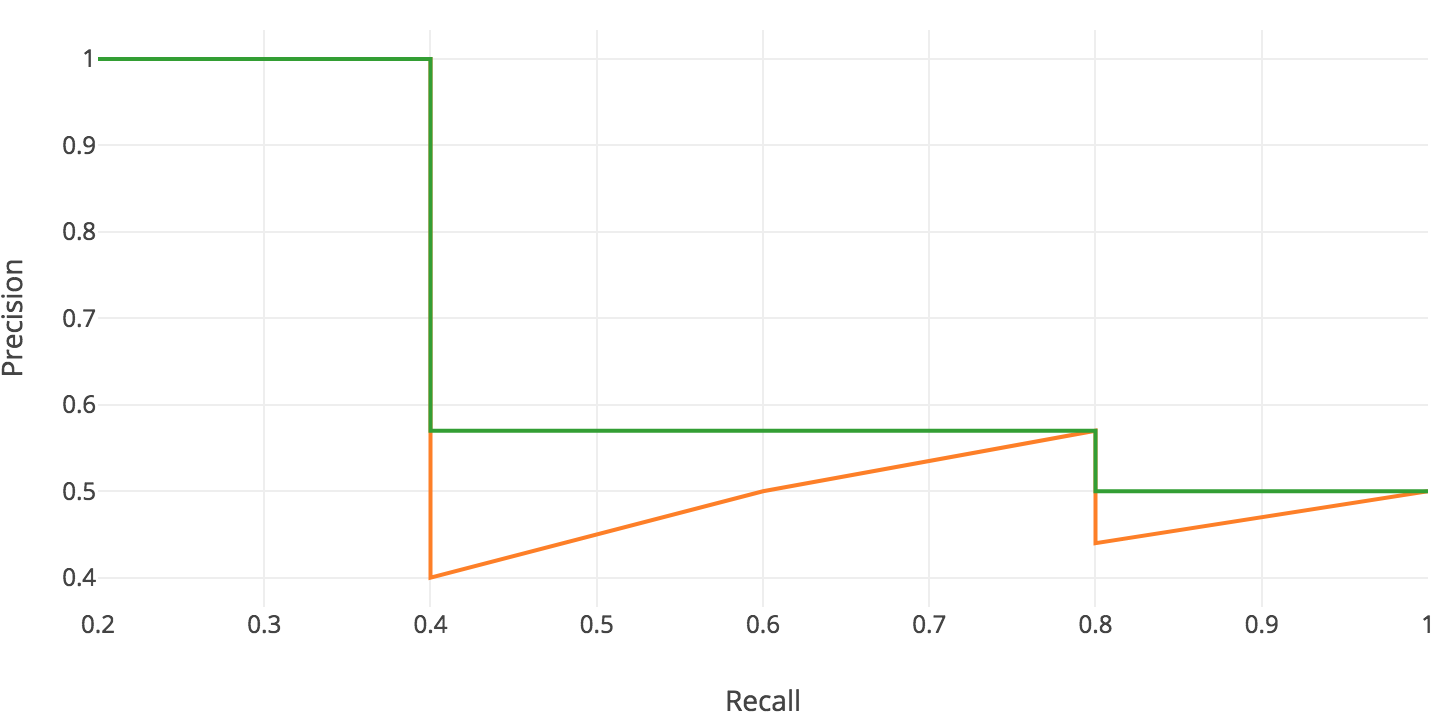
\includegraphics[width=0.5\textwidth]{Figures/mAP.png}
	\caption[Caption for figure in TOC.]{Example of precision/recall curve, adapted from~\cite{mAP}}
	\label{fig:mAP}
\end{figure}

%The score of classification $k$ is defined as interpolated
%precision ($P_{inter}(k)$).
%
%%how to compute Pinter ?
%
%
%With the number of ground truth positives (GTP), the
%AP is calculated by
%
%%what is GTP?
%
%\begin{equation}
%AP = \frac{1}{GTP} \sum_{i = 0}^{N} P_{inter}(i),
%\label{eq:AP}
%\end{equation}
%%END FIX (FIXED) - acabei por adicionar uma imagem, para mim é 1000x melhor do que qualquer texto que eu escreva
%where N is the total number of classifications above the IoU level.

Tab.~\ref{tab:yolov3_performance_metrics} presents the mAP
for a 0.5 IoU threshold and respective inference time (in ms) for
multiple networks. The results were obtained using machines with an M40 or Titan
X Pascal GPUs~\cite{yolov3} as indicated. The results show that the
Yolov3 networks achieve an accuracy on pair with the best performing networks at
a fraction of their inference time. The different versions of the Yolov3
networks are related with the resolution of the input images, but all have the
network structure.

\begin{table}[!htb]
	\renewcommand{\arraystretch}{1.2} % more space between rows
	\centering
	\begin{tabular}{lcccc}
		\toprule
		Network           & $mAP_{50}$ & Time (ms) & FPS & GPU  \\
		\midrule
		SSD321		& 45.4	& 61 & 16.4 & M40\\
		DSDSD321	& 46.1	& 85 & 11.8& M40\\
		R-FCN		& 51.9	& 85 & 11.8& M40\\
		SSD513		& 50.4	& 125 & 8& M40\\
		DSSD513		& 53.3	& 156 & 6.4& M40\\
		FPN FRCN	& \textbf{59.1} & 172 & 5.8& M40\\
		RetinaNet-50-500 & 50.9	& 73 & 13.7& M40\\
		RetinaNet-101-500 & 53.1	& 90 & 11.1& M40\\
		RetinaNet-101-800 & 57.5	& 198 & 5.1& M40\\
		Yolov3-320 & 51.5	& \textbf{22} & \textbf{45.5}& Titan X Pascal\\
		Yolov3-416 & 55.3	& 29 & 34.5& Titan X Pascal\\
		Yolov3-608 & 57.9	& 51 & 19.6& Titan X Pascal\\
		\bottomrule
	\end{tabular}
	\caption[Table caption shown in TOC.]{mAP and inference time comparison between multiple networks, adapted from~\cite{yolov3, Focal_Loss}.}
	\label{tab:yolov3_performance_metrics}
\end{table}

\subsection{Yolov3}
\label{sec:yolov3}
As presented in Tab.~\ref{tab:yolov3_performance_metrics}, the Yolov3 network
performs object detection at a higher framerate than other networks, while
maintaining a comparable level of accuracy.

\begin{table}[!htb]
	\renewcommand{\arraystretch}{1.2} % more space between rows
	\centering
	\begin{tabular}{lc}
		\toprule
		Layer Type           & Number of Layers  \\
		\midrule
		Convolutional       & 75    \\
		Shortcut  			& 23     \\
		Route 			    & 4     \\
		Yolo  				& 3     \\
		Upsample 		    & 2     \\
		Total 				& 107 \\
		\bottomrule
	\end{tabular}
	\caption[Table caption shown in TOC.]{Yolov3 layer type composition.}
	\label{tab:yolov3_num_layers}
\end{table}
Tab.~\ref{tab:yolov3_num_layers} presents the layer composition of the Yolov3
network. The majority of the layers are convolutional. Most of the convolutional
layers are used for feature detection or for reducing the FM resolution. This network
uses convolutional layers with $3\times3$ kernels with stride 2 instead of
pooling layers.

Due to the depth of the network, shortcut layers are used, to tackle the
problems described in section ~\ref{subsection:shortcut_layer}.

The accuracy performance for small object detection also comes from using three
different cell grid scales as opposed to the two used in previous
versions~\cite{Yolov2_redmon2016yolo9000}: ($13\times13$), ($26\times26$) and
($52\times52$). The indicated resolutions are specific to the Yolov3-416
version.

Fig.~\ref{fig:yolov3_stages} presents the main stages that constitute recurring
sequences of layers in the network: the F stage presented in
Fig.~\ref{fig:F_Stage} and the Yolo stage presented in
Fig.~\ref{fig:Yolo_Stage}.

\begin{figure}[!htb]
	\begin{subfigmatrix}{2}
		\subfigure[F stage composition]{\label{fig:F_Stage} 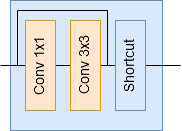
\includegraphics[width=0.25\textwidth]{Figures/FStage.png}}
		\subfigure[Yolo stage composition]{\label{fig:Yolo_Stage} 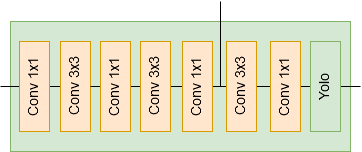
\includegraphics[width=0.50\textwidth]{Figures/YoloStage.png}}	
	\end{subfigmatrix}
	\caption{Stages of Yolov3 Network}
	\label{fig:yolov3_stages}
\end{figure}

Each F stage is composed of a convolutional layer with $1\times1$ kernels followed by
another with $3\times3$  kernels. At the end of the stage there is a shortcut layer
that adds the outputs of the second layer to the input of the stage.

In each Yolo stage, there is a sequence of convolutional layers, with $3\times
3$ and $1\times 1$ kernels that generate FMs of size $13 \times 13$ into the
first yolo layer. Since Yolov3 performs three detection attempts per grid cell,
there are $3\times 85 = 255$ FMs as input for every yolo layer. The
classification takes place for a grid with the same size as the FMs and the
number of FMs corresponds to the number os parameters to be calculated per grid
cell.

A complete scheme of the network is presented in Fig.~\ref{fig:Yolov3_complete}.

\begin{figure}[!htb]
	\centering
	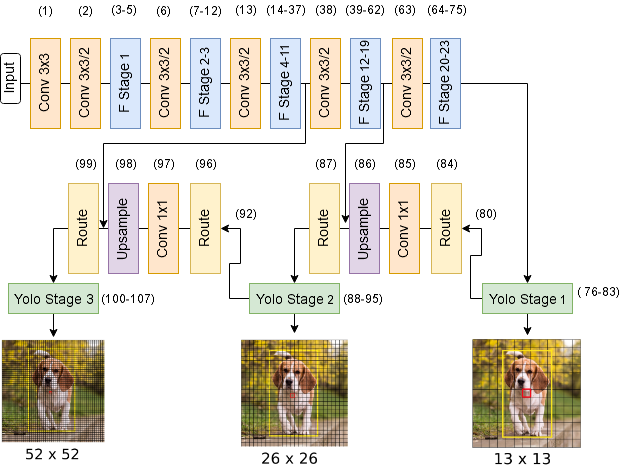
\includegraphics[width=0.85\textwidth]{Figures/CompleteYolov3Diagram.png}
	\caption[Caption for figure in TOC.]{Diagram of Yolov3 network}
	\label{fig:Yolov3_complete}
\end{figure}

The first part of the network is composed of a series of convolutional layers
terminated by F stages. Convolutional layers with stride 2 reduce the FMs by a
factor of four along the way. In this network implementation, the convolutions
use zero padding around the input FMs, so the size is maintained in the output
FMs. This part of the network is responsible for the feature detection in the
input image.

The second part of the netwok begins with a Yolo stage after which there is a
route layer that concatenates the output of the layers indicated in
Fig.~\ref{fig:Yolov3_complete}. This output is then compacted in terms of depth
by a $1\times 1$ convolution and upsampled by a factor of 2 in each FM
dimension, preparing the FMs for detections in a grid of $26\times26$ cells and
consequently detecting smaller objects in the image. These FMs are then
concatenated with the set of FMs of the same size from the detection part of the
network. The combination of the outputs of these two layers contribute with more
meaningfulness using the information from the upsampled layer and the
finer-grained information from the earlier feature maps~\cite{yolov3}.

After condensing the depth of the layer output to 255 FMs (again with a
convolutional layer with $1\times 1$ kernels), a second Yolo stage is used for
object detection at the new scale. The process is repeated one more time for the
third detection at the last yolo stage for a $52\times52$ grid.


\subsection{Tiny-YOLOv3}
\label{sec:tiny-yolov3}
For constrained environments, a small version of YOLOv3 is available. The layer
composition of the network is presented in
Tab.~\ref{tab:yolov3_tiny_num_layers}.

\begin{figure}[!htb]
	\begin{minipage}[b]{0.5\linewidth}
		\centering
		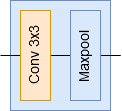
\includegraphics[width=0.35\textwidth]{Figures/TinyStage.png}
		\caption{Tiny-Yolov3 stage composition}
		\label{fig:Tiny_Stage}
	\end{minipage}%
	\begin{minipage}[b]{0.5\linewidth}
		\centering
		\begin{tabular}{lc}
			\toprule
			Layer Type           & Number of Layers  \\
			\midrule
			Convolutional       & 13    \\
			Maxpool  			& 6     \\
			Route 			    & 2     \\
			Yolo  				& 2     \\
			Upsample 		    & 1     \\
			Total 				& 24 \\
			\bottomrule
			
		\end{tabular}
		\caption[Table caption shown in TOC.]{Tiny-Yolov3 layer type composition.}
		\label{tab:yolov3_tiny_num_layers}
	\end{minipage}
\end{figure}

The first part of the network is composed of repeated Tiny-Yolov3 stages
presented in Fig.~\ref{fig:Tiny_Stage}. Each stage is composed of a
convolutional layer with $3\times3$ followed by a maxpooling layer.

This network follows the same sequence of layers present in Yolov3. The main
differences are in the number of layers and in the number of detections
performed. The Tiny-Yolov3 network performs object detection at only 2 grid
resolutions: $13\times13$ and $26\times26$.

\section*{Final Remark}
State-of-the-art CNN models are widely used for object detection
applications. These networks rely on convolution to extract features from the
images in order to be able to perform object detection. In order to achieve
higher performance metrics, CNNs grow in complexity. The Yolov3~\cite{yolov3}
network obtains comparable mAP for the COCO dataset~\cite{coco:Microsoft} to
other networks, at a fraction of the inference time.



 % file "Thesis_Background.tex"
%\cleardoublepage

%%%%%%%%%%%%%%%%%%%%%%%%%%%%%%%%%%%%%%%%%%%%%%%%%%%%%%%%%%%%%%%%%%%%%%%%
%                                                                      %
%     File: Thesis_CNNsOnFPGAs.tex                                     %
%     Tex Master: Thesis.tex                                           %
%                                                                      %
%     Author: Pedro Miranda                                            %
%     Last modified :  26 Dec 2019                                     %
%                                                                      %
%%%%%%%%%%%%%%%%%%%%%%%%%%%%%%%%%%%%%%%%%%%%%%%%%%%%%%%%%%%%%%%%%%%%%%%%

\chapter{CNNs in Reconfigurable Hardware}
\label{chapter:CNNs_on_FPGAs}

CNNs have been implemented on multiple devices, from CPUs and GPUs to
FPGAs. CPUs and GPUs mostly use temporal architectures, while FPGAs, which are
in the class of reconfigurable hardware devices use spatial architectures to
achieve parallelization. Another type of reconfigurable hardware devices is the
Coarse Grained Reconfigurable Array (CGRA) architecture, which, despite
powerful, is not as studied as FPGAs for the implementation of CNNs, and is the
main focus of this work.

An effective parallelization is specially important in the convolutional layers
which are responsible for $90\%$ of the execution time during inference
\cite{hal:accelCNNonFPGA}.

This chapter focusses on the main techniques used to accelerate convolutional
layers in Reconfigurable Hardware. First, the inherent parallelisms of the
convolutional algorithm are highlighted, followed by a presentation of the main
optimization techniques used. Closing the chapter, the Deep Versat CGRA, which
will be used in this work, is reviewed.

\section{General CNN Algorithm}
\label{sec:data_and_general_CNN_algorithm}
The data used in a convolution is presented in
Fig.~\ref{fig:data_representation}. A particular layer has an input $X$ composed
of $C$ FMs of size ($W\times H$) and uses $N$ kernels ($\Theta_1$ to $\Theta_N$)
of size ($J\times K \times C$) to obtain the output $Y$ composed of $N$ FMs of
size ($V\times U$). The generic CNN algorithm is presented in
Alg.~\ref{alg:general_CNN}. The bias is not represented for simplicity.
%The output $Y$ of a particular layer is obtained using the input $X$ and the
%kernels $\Theta_1$ to $\Theta_N$ in the generic CNN algorithm presented in
%Alg.~\ref{alg:general_CNN}. The bias is not represented for simplicity.

\begin{figure}[!htb]
	\centering
	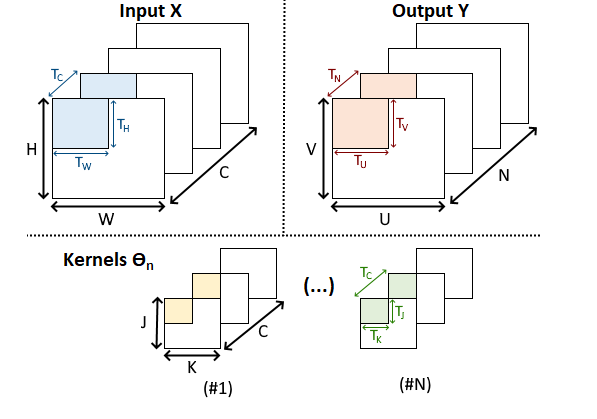
\includegraphics[width=0.5\textwidth]{Figures/data_representation.png}
	\caption[Caption for figure in TOC.]{Input pixels, kernels and output pixels representation, adapted from \cite{hal:accelCNNonFPGA}}
	\label{fig:data_representation}
\end{figure}

\begin{algorithm}
	\caption{General CNN algorithm for a single layer.}
	\label{alg:general_CNN}
	\begin{algorithmic}
		\FOR[\ // Loop 4 iterates over the $N$ channels of output $Y$]{$n \in \{1, \dots, N\}$} 
		\FOR{$v \in \{1,\dots,V\}$}
		\FOR[\ // Loop 3 iterates over the pixels within the same output FM]{$u \in \{1,\dots,U\}$} 
		\FOR[\ // Loop 2 iterates over the channels of input $X$]{$c \in \{1,\dots,C\}$} 
		\FOR{$k \in \{1,\dots,K\}$}
		\FOR[\ // Loop 1 iterates over a 2D kernel window]{$j \in \{1,\dots,J\}$}
		\STATE MACC: $Y[u, v, n] += X[j, k, c] \times \Theta_n [j, k] $
		\ENDFOR
		\ENDFOR
		\ENDFOR
		\ENDFOR
		\ENDFOR
		\ENDFOR	
	\end{algorithmic}
\end{algorithm}

The commented loops are candidates for loop unrolling, as discussed in section~\ref{sec:loop_unrolling}.
%Alg.~\ref{alg:general_CNN} has four different types of loops.
%\begin{itemize}
%	\item Loop 4 iterates over the $N$ channels of output $Y$.
%	\item Loop 3 iterates over the pixels within the same output FM.
%	\item Loop 2 iterates over the channels of input $X$.
%	\item Loop 1 iterates over a 2D kernel window.
%\end{itemize}


%The algorithm has four different parallelization opportunities, one for each of the commented loops in Alg.~\ref{alg:general_CNN}.
%\begin{itemize}
%	\item Loop 4 exhibits \underline{Inter-FM parallelism}, meaning that each output FM can be calculated in parallel. For each output FM the same input pixels are used, but a different kernel $\Theta_n$ is required.
%	\item Loop 3 presents \underline{Intra-FM parallelism} by calculating multiple output pixels within the same FM. This process uses the same kernel $\Theta_n$, but different input pixels.
%	\item Loop 2 highlights \underline{Inter-convolution parallelism} as each 3D convolution can be described as a sum of multiple 2D convolutions across the input FMs. Each 2D convolution requires different data from the input and kernel.
%	\item Loop 1 reveals \underline{Intra-convolution parallelism} as each 2D convolution at the two innermost loops can be implemented concurrently. As happens for Loop 2, there is no common data used at each Loop 1 iteration.
%\end{itemize}

 %Loop 4 exhibits \underline{Inter-FM parallelism}, meaning that each output FM can be calculated in parallel. For each output FM the same pixels are used, but a different kernel $\Theta_n$ is required. Loop 3 presents \underline{Intra-FM parallelism} by calculating multiple output pixels within the same FM. This process uses the same kernel $\Theta_n$, but different input pixels. Loop 2 highlights \underline{Inter-convolution parallelism} as each 3D convolution can be described as a sum of multiple 2D convolutions across the input FMs. Each 2D convolution requires different data from the input and kernel. Loop 1 reveals \underline{Intra-convolution parallelism} as each 2D convolution at the two innermost loops can be implemented concurrently. As happens for Loop 2, there is no common data used at each Loop 1 iteration.

\section{CNN Inference Acceleration in FPGAs}
\label{sec:CNN_inference_acceleration}
In general, acceleration for CNN inference in FPGA is done by a combination of \underline{datapath} and \underline{CNN model} optimizations.
%The algorithmic optimizations consist in transforming the convolution into either a general matrix multiplication (GEMM) or resorting to a Winograd transformation or Fast Fourier Transform (FFT).

Datapath optimizations explore parallelism opportunities in the convolutional algorithm described in~\ref{sec:data_and_general_CNN_algorithm}. However due to resource limitations in the devices when compared with the amount of calculations done in a single convolutional layer, only some parallelisms can be explored.

The last optimization type consists in trading model accuracy to improve computational and energy efficiency. This can be achieved by operating over reduced precision operands or reducing the model size.

% FPGA acceleration techniques:
%	Algorithmic
%	Datapah Optimization
%	CNN Model optimization
%	HW Generation (dont talk about this)
% describe what I will use: Datapath and Quantization (Fixed Point)

%\section{Algorithmic Optimizations}
%\label{sec:Algorithmic_Opt}
%The GEMM is commonly used in CPUs and GPUs, having large memory requirements to replicate the kernels into matrix form. Implementations in FPGA avoid replicating the kernels by generating the access pattern of the convolution.
%
%The FFT transform is interesting for convolutions with kernels with size over ($5 \times 5$) \cite{hal:accelCNNonFPGA}, which are increasingly less common as networks for image processing tend to have $3 \times 3$ kernels.
%
%The Winograd transform presents particular efficiency for kernels with size equal or smaller than ($3 \times 3$), by reducing the amount of multiplications done in exchange for more additions. In FPGAs, the multiplications and additions have the same computational cost if the MACs are done exclusively in DSP blocks. In fact, with the Winograd transform, the total number of operations increases, making it less efficient than the regular convolution algorithm.% Furthermore, this method requires complex processing of the weights before inference deployment.\\

\section{Datapath Optimizations}
\label{sec:Datapath_Optimizations}
%The resource limitations of FPGA devices when contrasted with current CNNs, make the complete exploitation of all parallelisms referenced in \ref{sec:data_and_general_CNN_algorithm} impossible. 
In~\cite{hal:accelCNNonFPGA}, SIMD accelerators are presented as the main strategy for implementing datapath optimizations. The architecture of a generic SIMD accelerator is presented in Fig.~\ref{fig:SIMD_accel}. SIMD accelerators receive the input FMs and weights from external memory into an on-chip buffer. This data is then processed in a pool of PEs that output the results into an output buffer. The output is then sent back to the external memory. Each PE contains on-chip registers and performs the computations using DSP blocks.
%this paragraph comes from the (3.5) Memory Accesses in CNNs section, now commented
The two levels of caching implemented by the on-chip buffers and registers reduce the accesses to external memory. This reduction has a significant impact in terms of power consumption, since the accesses to external memory are the determinant factor for power consumption in FPGAs~\cite{sze:dnn_tutorial, hal:accelCNNonFPGA}.

%The main strategies used resort to SIMD accelerators. SIMD accelerators, Fig.~\ref{fig:SIMD_accel}, receive the input FMs and weights from external memory into a buffer. This data is then send to a pool of PEs that output the results into an output buffer. The output is then sent back to the external memory. Each PE contains on-chip registers and perform the computations using DSP blocks.

%The datapath optimization consists in finding the architectural configuration
%that maximizes the computational throughput.
With this accelerator architecture, the process of datapath optimization consists in finding the configuration of the PEs and data schedule that maximizes computational throughput, specially for convolutions.

Since the convolution is a set of nested loops (Alg.~\ref{alg:general_CNN}),
loop optimization techniques as \underline{loop unrolling}, \underline{loop
  tiling} and \underline{loop interchange} are applied.


\begin{figure}[!htb]
	\centering
	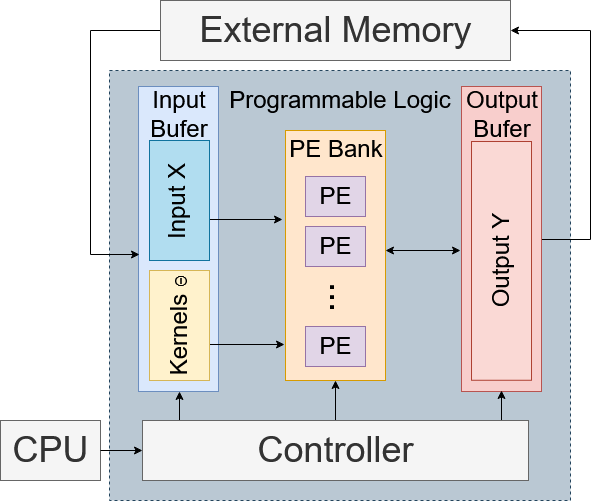
\includegraphics[width=0.5\textwidth]{Figures/SIMDAccelerator.png}
	\caption[Caption for figure in TOC.]{SIMD Accelerator, adapted from~\cite{hal:accelCNNonFPGA}}
	\label{fig:SIMD_accel}
\end{figure}

\subsection{Loop Unrolling}
\label{sec:loop_unrolling}
%In Alg.~\ref{alg:general_CNN} there are four highlighted loops that lead to
%different dataflows.
In Alg.~\ref{alg:general_CNN}, there are four parallelization opportunities, one for each of the commented loops, each one leading to a different dataflow.


\begin{itemize}
	\item Loop 4, which iterates over the output channels, exhibits \underline{Inter-FM parallelism}, meaning that each output FM can be calculated in parallel. For each output FM the same input pixels are used, but a different kernel $\Theta_n$ is required. By unrolling loop 4, at each cycle, the same pixel is multiplied by a corresponding
	weight from different kernels. This leads to an uniform access for input pixels
	and kernels. All computed values belong to pixels in different output FMs, so
	all of them need to be stored for the next cycle.
	\item Loop 3, which iterates over the pixels within the same output FM, presents \underline{Intra-FM parallelism} by calculating multiple output pixels within the same FM. This process uses the same kernel $\Theta_n$, but different input pixels. Unrolling Loop 3 requires accessing different pixels within the same FM, but
	enables the reuse of the weights. All the computed values belong to a different
	output pixel, so the number of partial values that need to be stored corresponds
	to the unroll factor applied to this loop.
	\item Loop 2, which iterates over the input channels, highlights \underline{Inter-convolution parallelism} as each 3D convolution can be described as a sum of multiple 2D convolutions across the input FMs. Each 2D convolution requires different data from the input and kernel. Unrolling Loop 2 leads to an uniform access for input pixels and weights in input FM and 2D kernel coordinates. However each value pair comes from a different
	channel. All the calculated values can be added into a single partial sum.
	\item Loop 1, which iterates over a 2D kernel window, reveals \underline{Intra-convolution parallelism} as each 2D convolution at the two innermost loops can be implemented concurrently. As happens for Loop 2, there is no common data used at each Loop 1 iteration. Unrolling Loop 1 requires accessing different input and weight positions at the
	same channel. This requires a complex address generation. All the calculated
	values are used for the same output pixel, therefore can be added, requiring the
	storage of only one partial sum value.
\end{itemize}
%Unrolling Loop 1 requires accessing different input and weight positions at the
%same channel. This requires a complex address generation. All the calculated
%values are used for the same output pixel, therefore can be added, requiring the
%storage of only one partial sum value.
%
%Unrolling Loop 2 leads to an uniform access for input pixels and weights in (x,
%y) and (j, k) coordinates. However each value pair comes from a different
%channel. All the calculated values can be added into a single partial sum.
%
%Unrolling Loop 3 requires accessing different pixels within the same FM, but
%enables the reuse of the weights. All the computed values belong to a different
%output pixel, so the number of partial values that need to be stored corresponds
%to the unroll factor applied to this loop.
%
%For loop 4, at each cycle, the same pixel is multiplied by a corresponding
%weight from different kernels. This leads to an uniform access for input pixels
%and kernels. All computed values belong to pixels in different output FMs, so
%all of them need to be stored for the next cycle.
%
%The chosen method of loop unrolling influences the parallelism scheme used and
%the number of multipliers required.

\subsection{Loop Tiling}
\label{sec:loop_tiling}
Loop tiling is used if the input data in deep CNNs is too large to fit in the on-chip
memory at the same time~\cite{hal:accelCNNonFPGA}. Loop tiling divides the data into blocks, like in
Fig.~\ref{fig:data_representation}, that are placed in the on-chip memory. The
main goal of this technique is to assign the tile size in a way that leverages
the data locality of the convolution and minimizes the data transfers from and
to external memory. Ideally, each input and weight is only transferred once from
external memory to the on-chip buffers.

If the kernel size is bigger than the stride ($J>Stride\text{ or }K>Stride$),
the resulting tiles overlap each other at the boundaries. The added amount of
reads is negligible when compared with the tile area~\cite{Ma:80_OptDataflow_in_CNN}.

The tiling factors set the lower bound for the size of the on-chip buffer.

\subsection{Loop Interchange}
\label{sec:loop_interchange}
Loop interchange sets the execution order of the four loops. The innermost loop
is the first to be computed and the outermost loop is the last to be completed.

The loop interchange can be divided into intra-tiling and inter-tiling loop
order. The intra-tiling loop order determines the dataflow from the on-chip
memory to the PEs, since the data belongs to the same tile loaded into the
on-chip buffer. While the inter-tiling loop order sets the dataflow from
external memory to the on-chip memory, by defining the order of the tiles loaded
into the on-chip buffer.

\subsection{Design Space Analysis}
\label{sec:datapath_opt_analysis}
In~\cite{Ma:80_OptDataflow_in_CNN}, the loop optimization techniques presented in sections~\ref{sec:loop_unrolling} to~\ref{sec:loop_interchange} are used to perform an analysis of the SIMD accelerators design space.


The development of the accelerator in~\cite{Ma:80_OptDataflow_in_CNN} is guided by the minimization of the
\underline{computing latency}, the requirements of \underline{partial sum
  storage} and the accesses to the \underline{external memory} and
\underline{on-chip buffer}.

The computing latency has a lower bound determined by the number of multipliers
available. However, if the ratios between the loop tiling factors and unroll
factors are not integers, the amount of multiplications done in parallel are less than the number of available multipliers. 
%FIX; what is underutilized in this case ???? bandwidth?
The same
happens if the ratio between the total data size and the tile size is not
integer with regards to the external memory transactions. 
% END FIX (FIXED)
To avoid the
underutilization of the resources, the chosen loop tiling factors should be
common factors of the total data size, the same needs to happen between the loop
tiling and unrolling factors.

The amount of partial sums that need to be stored depends mainly on the order of
loop computations. To reduce the number of stored partial sums the output pixel
values need to be computed as early as possible. This corresponds to having Loop
1 as the innermost loop.

The accesses to the external memory are tied to the size of the on-chip buffers,
which in turn have a size lower bound determined by the loop tiling factors.

The accesses to the on-chip buffers can be reduced by reusing the data sent to
the PEs. According to the analysis in~\ref{sec:loop_unrolling}, this corresponds
to unrolling Loop 3 and Loop 4.

\subsection{FPGA Implementation}
\label{sec:proposed_accelerator}
In~\cite{Ma:80_OptDataflow_in_CNN}, an accelerator architecture is implemented based on the impact of the loop optimizations in performance.

The accelerator proposed in~\cite{Ma:80_OptDataflow_in_CNN} unrolls loops 3 and 4, which minimizes the
on-chip memory accesses.

The tilling is done across W and H of the input data and V and N of the output
data. This tiling choice guarantees that the data for Loop 1 and Loop 2 is
always buffered and can be computed in sequence. In turn, this reduces the
amount of saved partial sums to the product of the unrolling
factors. Furthermore, the row tiling at the output requires sequential memory
accesses which benefit from DMA data transfers.

Tab.~\ref{tab:Ma_comparison} presents a comparison between the works
in~\cite{Ma_comp_ref10, Ma_comp_ref9, Ma_comp_ref8, Ma:80_OptDataflow_in_CNN},
which implement the VGG~\cite{VGG} network in FPGA.

The proposed accelerator in~\cite{Ma:80_OptDataflow_in_CNN} achieves over three
times the throughput of the other accelerators. The results highlight the impact in
computational throughtput of the datapath optimization strategies. For example, between implementations~\cite{Ma_comp_ref8} and~\cite{Ma:80_OptDataflow_in_CNN}, 
the same network, at the same frequency achieves over three times the throughput.
%The main difference between the
%accelerators is the datapath optimization strategy.

%Although the exact number of used DSP blocks and on-chip memory is not known
%for two of the implementations, the

\begin{table}[!htb]
	\renewcommand{\arraystretch}{1.2} % more space between rows
	\centering
	\caption[Table caption shown in TOC.]{Comparison of CNN FPGA implementations, adapted from~\cite{Ma:80_OptDataflow_in_CNN}}
	\label{tab:Ma_comparison}
	\begin{threeparttable}
	\begin{tabular}{|c|c|c|c|c|}
		\hline
		Network [Implementation]     & VGG~\cite{Ma_comp_ref10}	& VGG~\cite{Ma_comp_ref9} & VGG~\cite{Ma_comp_ref8} & VGG~\cite{Ma:80_OptDataflow_in_CNN}  \\ \hline
		FPGA      			 & Zynq XC7Z045 & Stratix-V GSD8 & Virtex-7 VX690t & Arria-10 GX 1150    \\  \hline
		Frequency (MHz)		& 150			& 120			&150				&	150			\\  \hline
		%\# Operations (GOP)  	 & 	30.76		&	30.95		&	30.95			&30.95				\\   \hline
		Number of Weights	& 50.18 M		&	138.3 M		&138.3 M			&138.3 M				\\  \hline
		%Precision (all fixed) & 16 bit		&	8 - 16 bit	&	16 bit			&8 - 16 bit				\\  \hline
		DSP Utilization 	& 780 (89\%)	& 1,963\tnote{b}		&	3,600\tnote{b}			&1,518 (100\%)				\\  \hline
		%Logic Utilization  & 				&				&					&				\\  \hline
		On-chip RAM\tnote{a}			& 486 (87\%)	& 2,567\tnote{b}		&1,470\tnote{b}				&1,900 (70\%)				\\  \hline 
		Latency/Image (ms) & 224.6			&262.9			&151.8				&47.97				\\  \hline
		Throughput (GOPS)	&136.97			&117.8			&203.9				&645.25				\\ \hline
		Unrolled Loops		& 1,2,4		& 1,2,4				& 1,2,4					& 3,4				\\ \hline
	\end{tabular}
		\begin{tablenotes}
	\item[a] Xilinx FPGAs in BRAMs (36 Kb) and Altera FPGAs in M20K RAMs (20 Kb)\\
	\item[b] The resource utilization is not reported in the original papers. The total available resources of the used FPGAs are listed
\end{tablenotes}
\end{threeparttable}
\end{table}


%\begin{table}[!htb]
%	\renewcommand{\arraystretch}{1.2} % more space between rows
%	\centering
%	\caption[Table caption shown in TOC.]{Comparison of CNN FPGA implementations, adapted from \cite{Ma:80_OptDataflow_in_CNN}}
%	\label{tab:Ma_comparison}
%	\begin{threeparttable}
%	\begin{tabular}{|c|c|c|c|}
%		\hline
%		Network           	& VGG 			& VGG			  & VGG  \\ \hline
%		FPGA      			 & Zynq XC7Z045 & Stratix-V GSD8  & Arria-10 GX 1150    \\  \hline
%		Frequency (MHz)		& 150			& 120				&	150			\\  \hline
%		%\# Operations (GOP)  	 & 	30.76		&	30.95				&30.95				\\   \hline
%		Number of Weights	& 50.18 M		&	138.3 M			&138.3 M				\\  \hline
%		%Precision (all fixed) & 16 bit		&	8 - 16 bit			&8 - 16 bit				\\  \hline
%		DSP Utilization 	& 780 (89\%)	& 1,963\tnote{b}		&1,518 (100\%)				\\  \hline
%		On-chip RAM\tnote{a}			& 486 (87\%)	& 2,567\tnote{b}		&1,900 (70\%)				\\  \hline 
%		Latency/Image (ms) & 224.6			&262.9			&47.97				\\  \hline
%		Throughput (GOPS)	&136.97			&117.8			&645.25				\\ \hline
%		Unrolled Loops		& 1,2,4		& 1,2,4		& 3,4				\\ \hline
%	\end{tabular}
%		\begin{tablenotes}
%			\item[a] Xilinx FPGAs in BRAMs (36 Kb) and Altera FPGAs in M20K RAMs (20 Kb)\\
%			\item[b] The resource utilization is not reported in the original papers. The total available resources of the used FPGAs are listed
%		\end{tablenotes}
%	\end{threeparttable}
%\end{table}


%\section{Mapping of Other Layers}
%\label{sec:mapping_other_layers}

\section{CNN Model Optimization}
\label{sec:CNN_model_opt}

The two most common methods for CNN model optimization in FPGA
devices are \underline{operand quantization}  and \underline{operation reduction}.
These methods reduce the amount of resources required, enabling more
parallelization and reducing the data transfers.

CNN model optimizations need to take into account the accuracy loss of the
model. In order to minimize the accuracy loss, these methods are integrated into
the model training phase.

%The CNN model optimization is implemented in FPGA devices by two main methods:
%\underline{operand quantization} or \underline{operation reduction}. These
%methods reduce the amount of resources required, which enables more
%parallelization and reduce the data transfers, which is the main factor for
%energy consumption.
%
%The performed approximations need to take in account the accuracy loss of the
%model. For further accuracy loss minimization, these methods are integrated into
%the training phase of the model.

\subsection{Quantization}
\label{sec:quantization}
Quantization is done by reducing the operand bit size. This restricts the
operand resolution, affecting the resolution of the computation
result. Furthermore, representing the operands in fixed-point instead of
floating-point translates into another reduction in terms of required resources
for computation.
% For example, a DSP block can perform two $18\times 19$ independent fixed point multiplications, while only being able to do one floating point multiplication.\\

The simplest quantization method consists in setting all weights and inputs to
the same format across all layers of the network. This is referred as static
fixed point (SFP). However, the intermediate values still need to be bit-wider
to prevent further accuracy loss.

In deep networks, there is a significant variation of data ranges across the
layers. The inputs tend to have larger values at latter layers, while the
weights for the same layers are smaller in comparison. The wide range of values
makes the SFP approach inviable, since the bit-width needs to expand to
accommodate all values.

This problem is addressed by Dynamic Fixed Point (DFP), which consists in the
attribution of different scaling factors to the inputs, weights and outputs of
each layer.

%The most common quantizations involve a linear mapping with uniform distance
%between each quantization level. Other common approaches use a simple mapping
%function like the log function that can be easily implemented in hardware.
%FIX este paragrafo é impossivel de perceber. Qual a relação entre distance e scale factor? Desde quando o log é facil de implementar em hw se ha teses de doutoramento sobre o assunto? (FIXED) - mais vale nem falar disto

In~\cite{Ma:ALAMO}, a DFP implementation with 8 bits for the weights and 10 bits
for the pixel values, without fine-tuning of the weights, is presented. The DFP
implementations yielded minimal accuracy losses for the networks tested, as is
presented in Tab.~\ref{tab:quantization_from_ALAMO}. The fixed-point precision
representation leads to an accuracy loss of less than 1\%.

\begin{table}[!htb]
	\renewcommand{\arraystretch}{1.2} % more space between rows
	\centering
	\begin{tabular}{|c|c|c|c|c|}
		\hline
		\textbf{\begin{tabular}[c]{@{}c@{}}Model Accuracy\\ Comparison\end{tabular}} & \multicolumn{2}{c|}{\textbf{\begin{tabular}[c]{@{}c@{}}Full \\ Precision\end{tabular}}} & \multicolumn{2}{c|}{\textbf{\begin{tabular}[c]{@{}c@{}}Fixed-Point \\ Precision\end{tabular}}} \\ \hline
		\textbf{CNN Model}                                                           & \textbf{Top-1}                             & \textbf{Top-5}                             & \textbf{Top-1}                                 & \textbf{Top-5}                                \\ \hline
		AlexNet~\cite{AlexNetKrizhevsky:2012}                                                                      & 56.78\%                                    & 79.72\%                                    & 55.64\%                                        & 79.32\%                                       \\ \hline
		NIN~\cite{NIN:cnnModel}                                                                          & 56.14\%                                    & 79.32\%                                    & 55.74\%                                        & 78.96\%                                       \\ \hline
	\end{tabular}
	\caption[Table caption shown in TOC.]{Accuracy Comparison with the ImageNet dataset, adapted from~\cite{Ma:ALAMO}}
	\label{tab:quantization_from_ALAMO}
\end{table}

\subsection{CNN Model Reduction}
\label{sec:CNN_prunning}
Another way to optimize the CNN model is to reduce the amount of computations
necessary for inference. One method to achieve this is through
\underline{weight pruning}. %Unlike
%quantization, CNN model reduction requires retraining of the weights.

Weight pruning consists in eliminating or zeroing the lowest weights. After
that, the remaining weights are fine-tuned in order to improve the
accuracy. Other criteria for pruning can be developed, like energy based
approaches. In~\cite{Yang_Energy-prunning} the energy consumption of each layers is estimated
by accounting for the accesses to the multiple memory levels and the energy expended for computation.
The amount of energy estimated by a layer determines the order in which the layers are pruned.
The more energy demanding layers are pruned first, since the first layers being pruned tend
to have better compression ratios than following layers.
%FIX se referes energy-based explica! (FIXED)

%The low rank approximation reduces the computation by replacing the convolution
%of a 3D kernel by three successive 1D filters. This
%is possible if the kernel has low rank to begin with, meaning that all the columns 
%in a 2D kernel are linearly dependent. The same for 
%With this alteration a 3D
%convolution requires $J+K+C$ multiplications instead of $J\times K\times C$. To obtain low rank
%kernels, the cost function during training can be altered to promote kernels
%with such characteristics. Another option is to approximate a kernel by a
%succession of low rank filters, resulting in $r\times (J+K+C)$ multiplications.
% FIX: o que é low rank? o que é J, K, C? (não vou virar a pagina para ver) Porque dá um resultado aproximado com muitas menos mults?
% paragrafo totalmente inaceitável : ou explicas ou apagas (FIXED) - isto até é muito interessante, mas levava a uma explicação alongada que também não é o foco do trabalho

Tab.~\ref{tab:model_reduction_comp} presents results achieved by CNN model
reduction techniques. Both implementations manage to remove the majority of the
weights without significant impact in accuracy. In
fact,~\cite{Hal_model_reduction_ref45,
  Hal_model_reduction_ref7} claim an accuracy reduction within 1\% when compared
with the respective model using all parameters.
% FIX all implementations como se a primeira é Low rank? Ou será low Rank + Prunning? São todas os só as Pruning? 
%(FIXED) - como não falo de SVD/low rank também não incluo na tabela


\begin{table}[]
	\centering
	\begin{tabular}{|l|c|c|c|c|}
		\hline
		\multicolumn{1}{|c|}{\textbf{Optimization}} & \textbf{Dataset}  & \textbf{Removed Parameters (\%)} & \textbf{Accuracy (\%)} & \textbf{Bitwidth}       \\ \hline
%		Low rank~\cite{Hal_model_reduction_ref9}                           & ImageNet & 63.6                    & 87.96         & 16 Fixed Point \\ \hline
		Prunning~\cite{Hal_model_reduction_ref45}                           & Cifar10  & 89.3                    & 91.53         & 8 Fixed Point  \\ \hline
		Prunning~\cite{Hal_model_reduction_ref7}                           & ImageNet & 85.0                    & 79.70     & 32 Float       \\ \hline
	\end{tabular}
	\caption{Accuracy of implementations using CNN model reductions, adapted from~\cite{hal:accelCNNonFPGA}}
	\label{tab:model_reduction_comp}
\end{table}

%\section{Memory Accesses in CNNs}
%\label{sec:Memory_accesses_CNNs}
%The accesses to external memory require more energy than computation by several orders of magnitude~\cite{sze:dnn_tutorial, hal:accelCNNonFPGA}. The number of accesses to external memory is reduced via the implementation of a caching hierarchy using on-chip buffers. Typically, two levels are used: one at the accelerator level and small register banks at the Processing Element (PE) level.

%Due to the locality in the data used in convolution operations, the memory accesses can be done in parallel with the computation. Dividing the on-chip buffers into two parts: one for the data being used in the current calculation and other to be loaded from memory for the next calculation at the same time. This is specially relevant for the execution of fully-connected layers due to their increased amount of weights. 



%In FGPAs, the bottleneck comes from the memory accesses since a MAC requires multiple reads for input (weight, input feature map and partial sum) and one write (new partial sum).
%
%%insert small figure of MAC
%This bottleneck goes hand to hand with the energy efficiency of the devices, since the memory accesses require more energy than computation by several orders of magnitude \cite{sze:dnn_tutorial, hal:accelCNNonFPGA}. The bottleneck is reduced via the implementation of on-chip buffers at the accelerator level and small register banks at the Processing Element (PE) level, where the MACs are performed.
%
%Due to the locality in the data used in convolution operations, the memory accesses can be done in parallel with the computation. Dividing the on-chip buffers into two parts: one for the data being used in the current calculation and other to be loaded from memory for the next calculation at the same time. This is specially relevant for the execution of fully-connected layers due to their increased amount of weights. 
% dont focus too much more on energy for now

\section{Coarse Grained Reconfigurable Arrays}
\label{sec:CGRAs_Versat}
Coarse Grained Reconfigurable Arrays (CGRAs) are presented
in~\cite{CGRA:Overview2016_wijtvliet} as middle ground between FPGAs and general
purpose processors (GPPs). In fact, a tendency from both FPGAs and GPPs towards
CGRAs is highlighted: on the one hand FPGAs tend to have more coarse grained
blocks like DSPs, while GPPs become more heterogeneous to include special
instructions and accelerators.

In~\cite{CGRA:Overview2016_wijtvliet}, CGRAs are defined as having temporal
granularity at the region level or above (Fig.~\ref{fig:time_granularity}) and
spatial granularity at the fixed functional unit (FU) level or above
(Fig.~\ref{fig:space_granularity}). As such, CGRAs are able to change the
architecture to fit the application during runtime.

\begin{figure}[!htb]
	\begin{subfigmatrix}{2}
		\subfigure[Spatial granularity levels]{\label{fig:space_granularity} 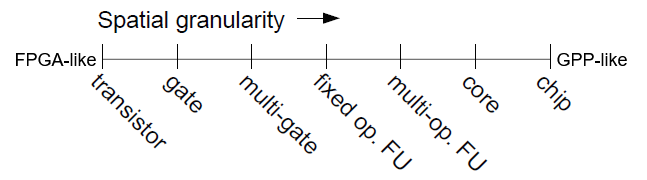
\includegraphics[width=0.49\textwidth]{Figures/Spatial_granularity_edited.png}}
		\subfigure[Temporal granularity levels]{\label{fig:time_granularity} 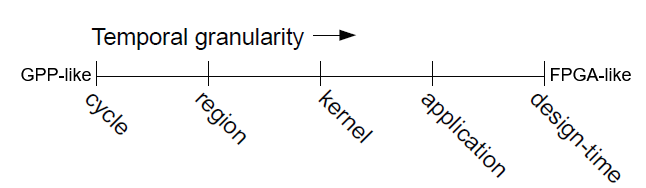
\includegraphics[width=0.49\textwidth]{Figures/Temporal_granularity_edited.png}}	
	\end{subfigmatrix}
	\caption{Spatial and temporal granularity levels, adapted from~\cite{CGRA:Overview2016_wijtvliet}}
	\label{fig:CGRA_granularities}
\end{figure}
CGRAs are integrated in systems mainly as accelerators. The runtime
reconfigurability allows for changes in the datapath, which allows for hardware
reuse in complex applications. At the same time, the FU granularity enables
enough degree of control for applications that do not take advantage of
bit-level manipulation.

With an adequate tool chain for assembly, compilation and place and route, CGRAs
have the potential to facilitate HW acceleration for multiple application types.

Neural networks is one of such applications. All layers in a neural network have
the same elemental operations which are mostly MACs and data
transfers. Therefore, with tailored FUs and correct datapath configuration, a
neural network acceleration environment based on CGRAs seems very attractive.
%One example are neural networks, which are composed of multiple layers. However, all layers have the same elemental operations which are mostly MACs and data transfers. Therefore, with tailored FUs and correct datapath configuration, a neural network acceleration environment based on CGRAs seems very attractive.
\section{Deep Versat}
\label{sec:Deep_Versat}
Deep Versat is a CGRA architecture proposed and implemented
in~\cite{VMario:Deep_Versat}. Deep Versat is composed by Versat Layers disposed
in a ring structure, as presented in Fig.~\ref{fig:DeepVersat_architecture}.

Each Versat Layer is composed of a Configuration Module (CM) and a Data Engine
(DE). This architecture provides a sustainable way to scale the Versat
architecture developed in~\cite{JDLopes:Thesis_Versat}. The scalability comes
from the fact that the inputs from a Versat Layer can select data from the same
Versat Layer or the previous one. With this connection policy, the routing
complexity is independent from the number of deployed Versat Layers.

\begin{figure}[!htb]
	\centering
	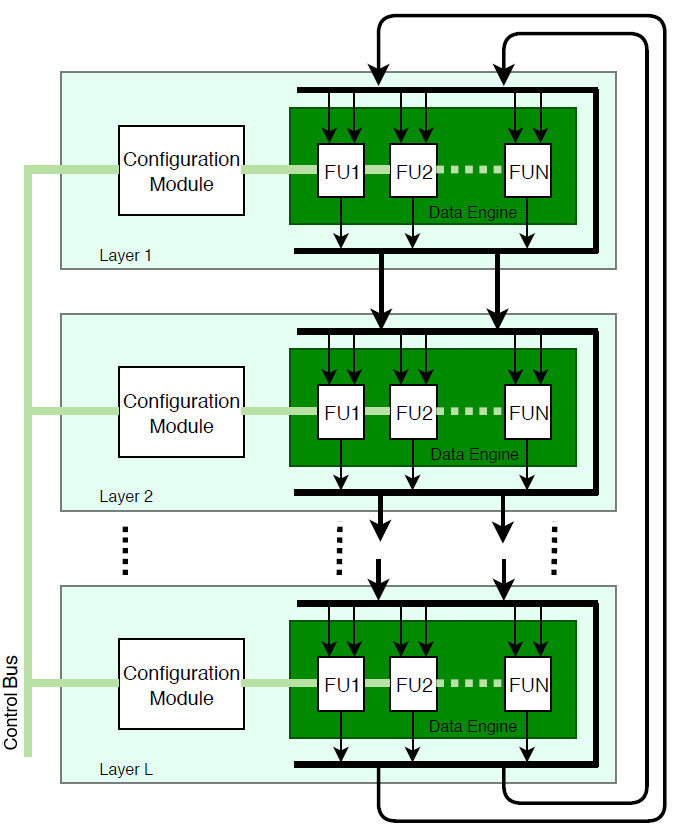
\includegraphics[width=0.5\textwidth]{Figures/deep_versat_arch.png}
	\caption[Caption for figure in TOC.]{Deep Versat architecture, from~\cite{VMario:Deep_Versat}}
	\label{fig:DeepVersat_architecture}
\end{figure}

\subsection{Data Engine}
\label{sec:versat_data_engine}
The Data Engine (DE) at each Versat Layer is where computations take place. The
DE is composed of a set of Functional Units (FUs) in a full-mesh topology. Even
though the number of FUs is variable, the topology presents scalability
problems, so the author recommends configuring the DE so that each FU input can
select one out of a maximum of 20 data sources (10 of then from the previous
Versat Layer). A diagram of a DE is presented in
Fig.~\ref{fig:Versat_data_engine}.

The DE also contains a Configuration Bus to configure each FU with the type
of operation and input selection.

The FUs in a typical DE are Arithmetic and Logic Units (ALUs), multipliers,
barrel shifters and dual-port embedded memories.

All FUs have a single output port with the exception of the dual-port memories,
which have two. The maximum number of FUs is 10, so that the Versat layer does
not produce more than 10 data sources that can be selected by the FUs
themselves.

The dual-port memories have two inputs and outputs and two Address Generation
Units (AGUs) that can generate addresses sequences for the two memory ports. The
AGUs are able to generate addresses for variables in nested double loops. Each
memory port can read from or write to an address generated by its AGU, an
address input to the other port, or can work as a Data Generation Unit (DGU),
outputting the sequence generated by the AGU to the memory port itself.

\begin{figure}[!htb]
	\centering
	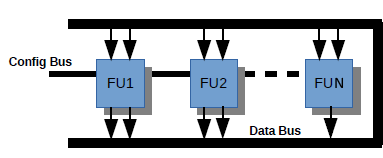
\includegraphics[width=0.5\textwidth]{Figures/versat_data_engine.png}
	\caption[Caption for figure in TOC.]{Versat data engine, adapted from~\cite{VMario:Deep_Versat}}
	\label{fig:Versat_data_engine}
\end{figure}


\subsection{Configuration Module}
\label{sec:versat_config_module}

The Configuration Module (CM) is the module where the DE configurations are
stored and managed. Fig.~\ref{fig:Versat_config_module} presents the structure
of the configuration module. The main components of this module are the
configuration memory, register file and shadow register.

The shadow register holds the configuration currently being executed by the
DE. The existence of this register allows for changes in the register file
without affecting the DE execution.

The configuration register file is composed of configuration spaces that in turn
have multiple configuration fields. One configuration field has the control bits
for a particular feature of a single FU, while a configuration space has the set
of configuration fields for an FU. Each configuration field can vary in bit
width as different the FU features require different numbers of configuration
bits. Configuration fields exploit time locality as the whole DE configuration
chages little over time. Furthermore, by being addressable at the configuration
field level, partial configuration of an FU becomes possible.

The register file takes advantage of time locality, as it is likely that the
same DE configuration is valid for a time span or similar configurations are
used in sequence.

The configuration memory can store 64 full DE configurations, the most used ones
usually, which can be loaded from or uploaded to the register file or external
memory, opening the possibility for more configuration storage in the system.
 

\begin{figure}[!htb]
	\centering
	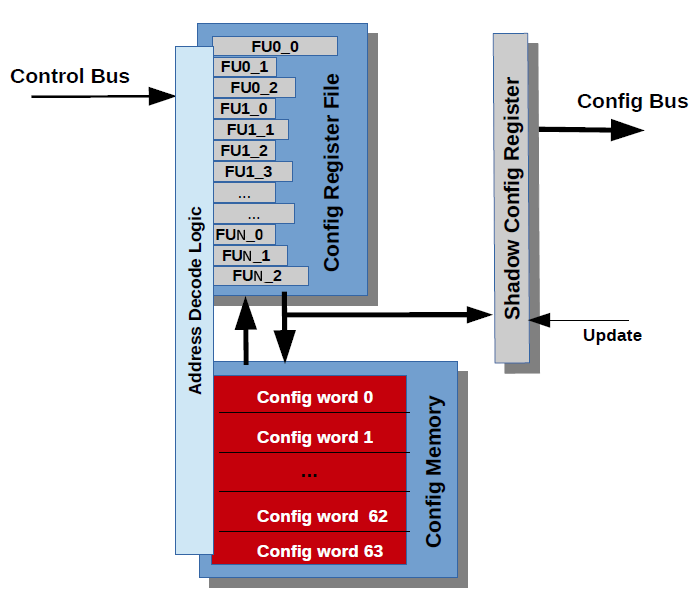
\includegraphics[width=0.5\textwidth]{Figures/versat_config_module_edited.png}
	\caption[Caption for figure in TOC.]{Versat configuration module, adapted from~\cite{JDLopes:Thesis_Versat}}
	\label{fig:Versat_config_module}
\end{figure}


\subsection{Controller and System Integration}
\label{sec:Versat_controller}
The Deep Versat layers are controlled by a soft processor using a RISC-V
architecture. This architecture is programmable with the GNU standard toolchain,
which contains compilers for C and C++.

In~\cite{VMario:Deep_Versat}, Deep Versat is connected to the controller as a
peripheral using the system control bus. It has a data interface connected
to a data bus. Each bus is memory mapped by a distinct memory base address.
There are also dataflow buses that connect two consecutive Versat layers.

The control bus is used to start a Deep Versat run and verify its
completion. Additionally, this bus can access the Versat memory FUs and is also
used to manage the configuration registers and memory.

The data bus connects Deep Versat to data sources and sinks and should be used
for larger and faster data transfers. The author comments on the inefficiency of
driving the data through the RISC-V processor and suggests the implementation of
a DMA engine connecting Deep Versat directly to the external memory instead.
 
Fig.~\ref{fig:DeepVersat_architecture} presents the system architecture, where
there is also a UART peripheral, used mainly for printing debug and verification
messages. Each Versat block represents a Versat layer of Deep Versat.

\begin{figure}[!htb]
	\centering
	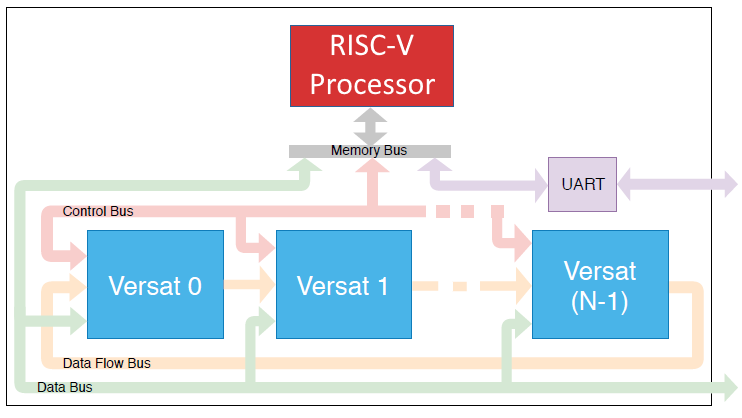
\includegraphics[width=0.6\textwidth]{Figures/deep_versat_system_edited.png}
	\caption[Caption for figure in TOC.]{Deep Versat system, adapted from~\cite{VMario:Deep_Versat}}
	\label{fig:deep_versat_system}
\end{figure}
\subsection{Deep Versat API}
\label{sec:Versat_API}
To facilitate datapath configuration in Deep Versat, an API in C++ was created
where the hardware modules are represented by classes and and their functions and
connections are accessed by the class's methods.

First, the definition of the number of Versat layers, types and number of FUs
and memory sizes is established. Then, the hardware architectural parameters of
Deep Versat are passed into the API via a python script that generates a C++
header file from the Verilog header file containing all the macros used for
pre-silicon configuration.


\section*{Final Remark}
\label{sec:chapter3_conclusion}
CGRAs have the potential to combine the computational capabilities of FPGAs with
the versatility of software, lowering the barrier of entry for model
deployment. For that, the CGRA requires dedicated FUs for the CNN layers that
exploit datapath and model reduction optimizations, while having an adequate
toolchain for software development.
 % file "CNNs on FPGAs"
%\cleardoublepage

%%%%%%%%%%%%%%%%%%%%%%%%%%%%%%%%%%%%%%%%%%%%%%%%%%%%%%%%%%%%%%%%%%%%%%%%
%                                                                      %
%     File: Thesis_Implementation.tex                                  %
%     Tex Master: Thesis.tex                                           %
%                                                                      %
%     Author: Andre C. Marta                                           %
%     Last modified :  2 Jul 2015                                      %
%                                                                      %
%%%%%%%%%%%%%%%%%%%%%%%%%%%%%%%%%%%%%%%%%%%%%%%%%%%%%%%%%%%%%%%%%%%%%%%%

\chapter{Proposed Work}
\label{chapter:implementation}

The proposed project consists in the development of a Yolov3 CNN application for
Deep Versat, with focus on the convolutional layer, that represents the majority
of computations in CNNs.

This involves the design of a set of acceleration datapaths for Deep Versat,
which, in turn, may require the improvement of the existing FU set. The overall
goal is to accelerate the execution of the application up to 30 images per
second in order to achieve video speed.

% intro to several sections

\section{Yolov3 Software Modeling}
\label{sec:yolov3_baseline}
The Yolo networks use Darknet~\cite{darknet13}, an open source neural network in
C and CUDA, which does not have support for reduced precision
operands. Therefore, the development of a code base that facilitates the
evaluation of the Yolov3 network in terms of operand precision becomes a
requirement.

This evaluation is necessary to verify the accuracy of the network with reduced
precision operands and to measure the ranges of the activations at each
layer. Only with this analysis it is possible to implement an effective
quantization based on DFP (section~\ref{sec:quantization}), which is necessary
for deep networks.


\section{Baseline Hardware System}
\label{sec:hw_baseline}
In order to establish a baseline for the performance of the Deep Versat, the
system presented in Fig.~\ref{fig:baseline_hw_system} will be used. The
architecture uses as base the system in~\cite{VMario:Deep_Versat}.

The main difference from the system in~\cite{VMario:Deep_Versat} is the addition
of the DMA connection between the Deep Versat and the external memory. As
discussed in~\ref{sec:Versat_controller}, this change frees the host system
during data transfers.

A RISC-V processor is used as the host and controller for Deep Versat. This soft
processor treats each other block in the system as a memory mapped
peripheral. The processor is also tasked to execute the parts of the application
that are not accelerated by the Deep Versat.

The UART block is useful in development for debugging purposes, as it is a
practical way to receive feedback from the system into a console on an external
computer.

Deep Versat has been programmed with a convolutional layer for accelerating a
hand written digit recognition application~\cite{VMario:Deep_Versat}. This
implementation uses Versat's current set of FUs, which are reconfigured many
times to form datapath configurations as discussed in~\ref{sec:Deep_Versat}.

With this implementation it is possible to both verify the correct functioning of
the system and all its components, as well as establishing a baseline in terms
of performance for convolution acceleration.

\begin{figure}[!htb]
	\centering
	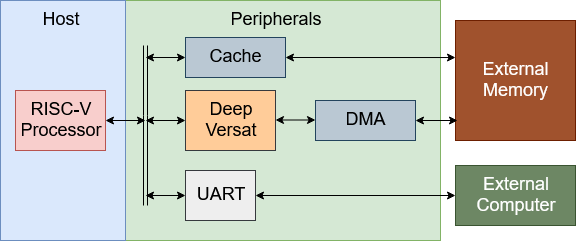
\includegraphics[width=0.6\textwidth]{Figures/baseline_HW_system.png}
	\caption[Caption for figure in TOC.]{Baseline hardware system}
	\label{fig:baseline_hw_system}
\end{figure}
%FIX o que liga o risc-v a memoria externa é uma cache e não um dma. Não existe Program Memory, é a cache. (FIXED)

\section{Datapath Proposal for Convolutional Layers}
\label{sec:planned_datapath_for_conv_layers}
The acceleration of convolutional layers will start with the proposal of a
datapath architecture, based on the analysis
in~\ref{sec:Datapath_Optimizations}. The accelerator presented
in~\ref{sec:proposed_accelerator} is a promising starting point for the
architecture.

The designed datapaths may require the development of new of FUs or tweaking of
the existing ones. There is then the challenge of mapping the convolution
datapaths into the Deep Versat architecture using the modified FU set.  After
that, the convolution layer can be tested and compared with the baseline
results. The work reported in this section is the main focus of the project and
is expected to be the most time consuming task.

\section{Experimental Validation with Yolo Networks}
\label{sec:experimental_yolo_validation}
With a new Convolutional Layer tested and working properly, the next test is to
execute the Tiny-Yolov3 network (section~\ref{sec:tiny-yolov3}) on the
system. This represents an intermediate step due to the reduced requirements of
this network, when compared with the full Yolov3. As a general goal for the
project, processing 30 images per second would be ideal, although this objective
may not be achieved.


%FIX: Não percebi porque é preciso desenvolver uma FU para conv. Já existe o MAC tal
%como explicaod no Alg1. O que podemos ter de mexer é nas AGUs para aumentar o
%numero de loops executados no Deep Versat


\section{Work Calendarization}
\label{sec:tasks_GANT}
In Fig.~\ref{fig:tasks_callendar} it is presented a GANT chart outlining the
calendarization of the planned work.


%FIX: altera o planeamento de acordo uma vez que não vejo a tarefa de desenhar uma FU como dominante.

\begin{figure}[!htb]
	\centering
	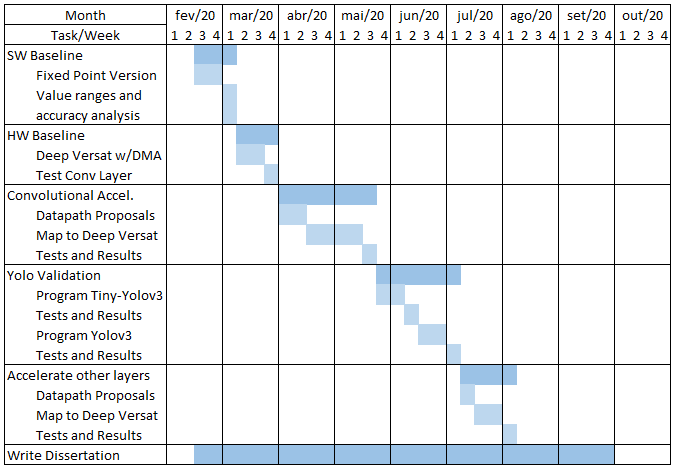
\includegraphics[width=0.95\textwidth]{Figures/dummy_GANT.png}
	\caption[Caption for figure in TOC.]{Work Planning}
	\label{fig:tasks_callendar}
\end{figure}


%\begin{itemize}
%	\item Proposed Methodologies
%	\subitem Outline of base system
%	\subitem PE in Versat architecture
%	\subitem General PE architecture proposal
%	\item Expected Results
%	\subitem Target performances and goals (accuracy, fps, networks)
%	\item Work planning table (GANT)
%\end{itemize}


 % file "Thesis_Implementation.tex"
%\cleardoublepage

%\input{Thesis_new_file} % add new .tex files for new chapters
% \cleardoublepage

%\input{Thesis_new_file} % add new .tex files for new chapters
% \cleardoublepage

%\input{Thesis_new_file} % add new .tex files for new chapters
% \cleardoublepage

%%%%%%%%%%%%%%%%%%%%%%%%%%%%%%%%%%%%%%%%%%%%%%%%%%%%%%%%%%%%%%%%%%%%%%%%%
%                                                                      %
%     File: Thesis_Results.tex                                         %
%     Tex Master: Thesis.tex                                           %
%                                                                      %
%     Author: Gonçalo Santos                                           %
%     Last modified : 20 Oct 2018                                      %
%                                                                      %
%%%%%%%%%%%%%%%%%%%%%%%%%%%%%%%%%%%%%%%%%%%%%%%%%%%%%%%%%%%%%%%%%%%%%%%%

\chapter{Results}
\label{chapter:results}

The aim of this work is to produce a workable {\bf C} language
compiler for the {\it Versat} architecture using the {\it picoVersat}
instruction set.
The success can be measured by the number of {\bf C} language
constructs that are working properly.
Consequently, testing is of primordial importance, as are the range
of tests used to exercise the compiler.

\section{Functionality}

The compiler, as far the tests were comprehensive,
supports all {\bf C} language integer constructs.
Limitations are listed below.

Since the processor instruction set is reduced, as are the
number of {\bf lcc} terminals to be implemented by the compiler,
the testing of each operation, on its own, is strait
forward.
Testing sequences of such operations may prove more
difficult to test, since different {\bf C} programs
can produce different selection matches.

\section{Testing}

In the test of a compiler, where a small change can affect the
generation of multiple instructions, a good set of
regressive tests is very important.
In order to automate the process, a {\tt test/} directory
was setup.
This directory includes a set of {\bf .c} test files and
the expected output {\bf .out}.

The {\tt Makefile} compiles, executes and compares the new
result with the previously stored result.
All differences in output are printed and can then be analyzed.

Since the output from {\bf iverilog} includes the number
of clocks spent, it is easy to compare whether the changes in the
compiler result in improvements, or in performance degradation.

Some tests are very simple and its output can be easily predicted.
To make testing even simpler, the return value of the {\tt main}
routine is printed, unless the {\sc NORET} environment variables
is defined. Upon return from the {\tt main} routine, the lowest
nibble is printed as an {\sc ASCII} starting at $0$.
This means that values between $10$ and $15$ are printed as
the {\sc ASCII} character at the respective offset, namely the
sequence: \verb|:|, \verb|;|, \verb|<|, \verb|=|, \verb|>|, \verb|?|.

More complex tests can be compiled with {\bf gcc} and executed
to access the expected output.
This, however, can not be performed if the examples include
{\tt asm} calls, since the code can only be executed by the
{\it Versat}, or by the {\bf iverilog} simulator, and not by the
native testbench processor.
%vdb.c

A set of $86$ regression tests is currently being used, ranging
from specific operator testing to complex recursive and iterative
examples. % And the number of tests keeps growing ...

\section{Limitations}\label{limitations}

The {\bf C} language imposes that {\tt sizeof(char)==1}
as does the {\bf lcc} compiler (see~\cite[p.79]{hanson95}).
This works fine as far as {\tt sizeof(char)} can be 32-bits.
However, additionally, the {\bf lcc} assumes through out
the code that $8$ is the number of {\em bit-per-byte}.
If it was a variable, one could set it to $32$.
As it is hardcoded, all address literals
will be truncated to 8-bits ({\tt 8}${}^{\wedge}${\tt ty->size}).
\begin{verbatim}
int *addr = (int*)0x123456;
\end{verbatim}
This can be avoided by setting an integer to the
required value and then assigning it to a pointer.
This works since integer literals are 32-bit wide
and the conversion to pointer, controlled by the
{\it back-end}, does not truncate the value.
\begin{verbatim}
int *addr, value = 0x123456;
addr = (int*)value;
\end{verbatim}
Nevertheless, defining literal pointer is never
a good predictive in virtual memory machines.
In {\it Versat} it is useful to map variables
to specific addresses.

Due to the same reason, a warning message is issued
({\tt shifting an `int' by 12 bits is undefined})
but the code is correctly generated.

% #define LONG_MIN -2147483648
% warning: unsigned operand of unary -
% but 0x80000000 or bellow is OK!
% #  define LONG_MAX	2147483647
% #  define LONG_MIN	(-LONG_MAX - 1L)

In the initial version of {\it picoVersat}, all global
data must be added by {\tt MEM\_BASE=512}.
Since this is performed when addresses are fetched,
static assignments store the unadded value.
Therefore, all accesses must be added by $512$.
Must add {\tt 512} to global pointers in {\tt picoversat-0.0}
\begin{verbatim}
int mem[10], *base = mem;
int main() { base[6+512] = 9; return return mem[6]; }
\end{verbatim}
This can be avoided if assignment is performed during
execution (not at compile time), even if the variable
is global.
\begin{verbatim}
int mem[10];
int main() { int *base = mem; base[6] = 9; return return mem[6]; }
\end{verbatim}

Signed multiplication, division and modulus ({\tt \_mul},
{\tt \_div} and {\tt \_mod}) do not generate carry since
the flags register of {\it picoVersat} is read-only.

The {\bf C} programming languages relies on separate
compilation, where several files are independently
compiled and then linked together.
However, there is no linker in the {\it Versat} system
and the assembler {\bf va} does not support multiple
files.
The solution is to perform linking with {\bf cpp} %%%
include directives.
While in normal {\bf C} the {\tt .c} should be
included, rather compiled, the inclusion of {\bf .h}
as well as {\bf .c} accomplishes the desired result.
Since there is no linking, only multiple inclusion
of files must be avoided.

The {\it Versat} architecture is meant to be used offline
and no form of argument passing to the {\tt main} routine
is available.
Consequently, the stack is initialized at the top.
Therefor, even if the program declares arguments to
the {\tt main} routine ({\tt argc, argv, envp}) they should
never be accessed.
Also, since the system has no memory management unit,
all illegal accesses are silently ignored by the system.
Highly recursive routines that exhaust the stack will have
unpredictable behaviors, since they will begin to overwrite
the top of the code.
Even if it is not the compilers responsibility, it something
that the programmer should be aware, especially when
transitioning from a virtual managed memory system.

Finally, the compiler does not support floating point
data types, since every operation must be supported
by library routines.
This is the case for many android devices, namely
smartphones.
However, the {\it Versat} purpose is to perform
integer arithmetic operations fast and is not aimed at
scientific programming.
The error message {\tt compiler error in \_label--Bad terminal}
is issued by the compiler when it cannot handle a given operation,
namely floating point operations.

\section{Register assignment}

Register assignment in compiler design considers two types of registers:
global registers that hold variable values and scratch registers that hold
temporary values.
The {\bf lcc} compiler defines these registers by setting a mask for each
type of register.
It is up to each {\it back-end} to define the mask values according to processor
capabilities.
For instance, the {\bf sparc} processor defines $4$ sets of $8$ registers:
global, temporary, input and output; where the later two sets replace
the stack for argument passing.
In {\bf i386} all $7$ registers are temporary, while {\bf mips} uses half
for each purpose ($16+16$).

Since the {\it picoVersat} has no specific register assignment, a study
was carried out in order to assess the best balance between global and
scratch registers.
Registers {\tt R0} and {\tt R13} to {\tt R15} are used to communicate with {\it Versat}
and are invisible to the compiler.
The stack is controlled by a {\it stack pointer} ({\tt R12}) and a {\it frame pointer}
({\tt R11}).
The remaining registers ({\tt R1} to {\tt R10}) compose a mask {\tt 7FE}, where
the lowest bit ({\tt R0}) is omitted for register assignment, and the highest
used bit {\tt 400} is {\tt R10}.
The register {\tt R1} is used to return function values and all arguments are
passed on the stack.
At least two registers must be used as scratch for binary operations
temporaries.
The compiler allows the definition of a {\tt tmask} for temporaries and a
{\tt vmask} for variables.

Initially, in run $1$, the experiment uses all registers for temporaries.
Each run adds a variable register at the expense of a temporary, until only
two temporaries remain (run $9$).
Three examples where used: {\tt assign}, {\tt repeating locals} and
{\tt bubble sort}.
The first two represent opposite extremes of register usage, while the last is
a more balanced and realistic example.

The first example uses the {\bf C} language right associative {\it assign} operator
where each new assignment to the variable {\tt a} requires a new temporary register.
%(see Figure~\ref{fig:assign}).

%\begin{figure}
\begin{verbatim}
int f() { return 1; }
int main()
{
  int a;

  a = f() + (a =
      f() + (a =
      f() + (a =
      f() + (a =
      f() + (a =
      f() + (a =
      f() + (a =
      f() + (a =
      f() + (a =
      f() + (a =
      f() + (a =
      f() + (a =
      f() + (a = 1
                  )))))))))))));
  return a;
}
\end{verbatim}
%\caption{}
%\end{figure}

The register usage shows that each assign uses a register $4$ times at
the expense of the return register {\tt R1}.
The best solution, represented by the lowest clock count,
is to use only two temporaries, since more variables imply more stack ({\tt R12}),
saves and restores between each call to the function {\bf f}.

%\begin{table}
\begin{center}
{\small
\begin{tabular}{r|r|r|r|r|r|r|r|r|r|r|r|r|r|r|r|r}
run&vars&vmask&tmask&R1&R2&R3&R4&R5&R6&R7&R8&R9&R10&R11&R12&clks\\\hline
1&0&000&7FE&21&4&4&4&4&4&4&4&6&44&27&82&677\\
2&1&400&3FE&23&4&4&4&4&4&4&6&42&17&14&82&638\\
3&2&600&1FE&25&4&4&4&4&4&6&42&0&17&16&77&633\\
4&3&700&0FE&27&4&4&4&4&6&42&0&0&17&18&72&628\\
5&4&780&07E&29&4&4&4&6&42&0&0&0&17&20&67&623\\
6&5&7C0&03E&31&4&4&6&42&0&0&0&0&17&22&62&618\\
7&6&7E0&01E&33&4&6&42&0&0&0&0&0&17&24&57&613\\
8&7&7F0&00E&35&6&42&0&0&0&0&0&0&17&26&52&608\\
9&8&7F8&006&39&42&0&0&0&0&0&0&0&17&28&47&603\\
\end{tabular}
}
\end{center}
%\caption{}
%\end{table}
\vspace*{5mm}

The second example uses lots of repeating local variables so that each one is assigned
a register, for its uses from the first to last line, if one is available.
%(see Figure~\ref{fig:locals}).

%\begin{figure}
\begin{verbatim}
int func(int a, int b, int c, int d, int e, int f, int g, int h, int i, int j, int k) {
    a = a + b - c - d - e + f - g + h + i + j + k;
    b = a - b + c + d - e - f + g - h + i - j - k;
    c = a + b - c - d + e + f + g - h + i + j - k;
    d = a - b - c + d - e + f - g + h - i - j - k;
    e = a + b + c - d - e - f - g + h - i + j - k;
    f = a - b - c + d - e + f + g - h - i - j + k;
    g = a + b - c - d + e + f + g - h + i + j - k;
    h = a - b + c + d - e - f - g + h + i - j - k;
    i = a + b - c - d - e + f + g + h + i + j - k;
    j = a - b - c + d - e + f + g - h - i - j - k;
    k = a + b + c - d + e - f - g - h - i + j + k;
    return a + b + c + d + e + f - g + h - i + j - k;
}

int main() {
    return func(10, 9, 8, 7, 6, 5, 4, 3, 2, 1, 0);
}
\end{verbatim}
%\caption{}
%\end{figure}

As expected, the best solution is to use highest of temporaries in order
to reduce frame pointer ({\tt R11}) accesses to stack saved values.

%\begin{table}
\begin{center}
{\small
\begin{tabular}{r|r|r|r|r|r|r|r|r|r|r|r|r|r|r|r|r}
run&vars&vmask&tmask&R1&R2&R3&R4&R5&R6&R7&R8&R9&R10&R11&R12&clks\\\hline
1&0&000&7FE&45&27&12&13&48&46&40&45&54&62&68&56&956\\
2&1&400&3FE&53&31&13&54&46&40&47&54&62&0&78&51&1001\\
3&2&600&1FE&61&35&52&46&48&49&56&62&0&0&89&46&1051\\
4&3&700&0FE&89&39&59&63&51&56&62&0&0&0&101&41&1106\\
5&4&780&07E&109&43&75&49&74&79&0&0&0&0&113&36&1161\\
6&5&7C0&03E&146&45&84&58&105&0&0&0&0&0&124&31&1211\\
7&6&7E0&01E&156&88&112&94&0&0&0&0&0&0&138&26&1278\\
8&7&7F0&00E&171&117&176&0&0&0&0&0&0&0&154&21&1356\\
9&8&7F8&006&231&249&0&0&0&0&0&0&0&0&172&16&1447\\
\end{tabular}
}
\end{center}
%\caption{}
%\end{table}
\vspace*{5mm}

The last example, the {\it bubble sort}, uses a mixture temporaries and variable
reuses. %(see Figure~\ref{fig:bubble}).

%\begin{figure}
\begin{verbatim}
#include "printi.h"

int bubble(int list[], int n) {
    int c, d, t, swap, cnt = 0;

    for (c = 0; c < n - 1; c++) {
        for (swap = 0, d = n - 1; d > c; d--)
            if (list[d - 1] > list[d]) {    /* Swapping */
                swap++;
                t = list[d];
                list[d] = list[d - 1];
                list[d - 1] = t;
            }
        if (!swap)
            break;
        cnt++;
    }
    return cnt;
}

int v[] = { 7, 4, 9, 6, 2, 1, 3, 5, 8, 0 };

int main() {
    int i, size = sizeof(v) / sizeof(v[0]), cnt = bubble(v, size);
    for (i = 0; i < size; i++) {
        putchar(v[i] + '0');
        putchar(' ');
    }
    printi(cnt, 10);
    putchar('\n');
    return 0;
}
\end{verbatim}
%\caption{}
%\end{figure}

This example exploits the tradeoff between global and temporary register
usage.
In the first runs the compiler is unable to use all temporaries.
In the last runs some variable registers are left unassigned and the number
of required execution clocks rises again.

%\begin{table}
\begin{center}
{\small
\begin{tabular}{r|r|r|r|r|r|r|r|r|r|r|r|r|r|r|r|r}
run&vars&vmask&tmask&R1&R2&R3&R4&R5&R6&R7&R8&R9&R10&R11&R12&clks\\\hline
1&0&000&7FE&2&0&0&0&0&4&5&15&30&45&31&36&9855\\
2&1&400&3FE&2&0&0&0&0&4&7&29&41&11&24&36&8193\\
3&2&600&1FE&2&0&0&0&4&5&27&37&7&11&19&41&7714\\
4&3&700&0FE&2&0&0&0&5&25&37&4&7&11&17&41&7399\\
5&4&780&07E&2&0&0&5&19&37&6&4&7&11&13&46&7022\\
6&5&7C0&03E&2&0&5&19&33&6&6&4&7&11&9&49&6949\\
7&6&7E0&01E&2&5&19&33&0&6&6&4&7&11&9&49&6949\\
8&7&7F0&00E&5&19&33&0&0&6&6&4&7&11&9&44&6921\\
9&8&7F8&006&21&28&0&0&0&6&6&4&7&11&13&41&7492\\
\end{tabular}
}
\end{center}
%\caption{}
%\end{table}
\vspace*{5mm}

Based on experience with the examples above, a balanced approach should work best
in most cases.
Therefor, the first five registers, {\tt R1} to {\tt R5}, are used as temporaries
({\tt tmask=0x003E}) and the remaining five, {\tt R6} to {\tt R10}, are used as
variables ({\tt vmask=0x07C0}).

\section{Efficiency considerations}

Calls are very expensive operations for any processor.
{\it Intel Inc.} has made a significant effort over the year to address this
problem.
In the last years, its high end processors provide faster {\it calls} than
{\it jumps} at the expense of higher transistor count. %ref!
In a processor like {\it picoVersat}, the problem is magnified since
no stack specific registers or opcodes are available.

A function call in the {\bf C} programming language requires:
\begin{enumerate} \itemsep0em 
\item {\bf argument passing} by pushing values to the stack;
\item {\bf calling} the desired routine;
\item {\bf saving used registers} before the routine destroys its values;
\item {\bf frame pointer} saving to access arguments and locals;
\item {\bf allocate space} for local variables;
\item actually performing the routine operations;
\item {\bf restoring frame pointer} of the previous routine;
\item {\bf restoring used registers} previous values;
\item {\bf returning} to the calling routine;
\item {\bf removing arguments} from stack.
\end{enumerate}
The present compiler detects when a routine accesses no arguments or locals
and does not emit frame pointer code. So, if a routine only uses global
variables, the call becomes a bit more efficient.
Some of the tests used become upto 5\% faster by removing the frame
pointer in routines where it not needed.

As any routine can be called many times, even recursively, the compiler
must save, at the beginning, and restore, at the end,
all the registers the routine uses.
This means that, at the start of the program, the {\tt main} routine will spill
all registers it will use, although they have no defined value.
Such procedure is required since the routine may be recursively called.
However, in most cases, the {\tt main} routine is only invoked once, at
the start of the program.
The {\sc NOSAV} environment variable can be set if the {\tt main}
routine is not used recursively and no registers will saved by the compiler.
This special hack can be dangerous to use, but it makes {\tt main} based
programs more efficient.

The {\it picoVersat} controls {\it Versat} by setting specific values to
predefined memory positions.
The use of a routine to perform such a task is a very
expensive way to change memory positions, either through {\tt asm}
directives or standard {\bf C} code, as the tests {\tt set.c} and
{\tt setvar.c} show, respectively.
Memory values can be efficiently changed by assigning to a pointer
{\tt *addr=val} (see Limitations, above).

During this work, the {\it picoVersat} evolved. The use of a single
memory, for program code and data, removed the need for a {\tt addi MEM\_BASE}
instruction for each variable load and store, resulting in a 5\% improvement
over all the regression test in use, at the time. % 17022/16213 pico-0

Finally, the compiler some times generates a register read after the
same register was written by another instruction selection.
At least, the read can be suppressed, but {\bf lcc} provides no
peephole optimizer for final code cleanup.

\section{Compiler instalation}

The compiler itself, {\bf lcc}, can be invoqued directly with the
{\tt -target=versat} option, as long as the input file has already
been preprocessed ({\bf cpp}).
The compiler output is a {\it picoVersat} assembly, that can then
fed to the {\it versat} assembler ({\bf va}).

However, the complete compilation process, from {\bf C} language
source file to {\bf iverilog} simulation executable, can be
integrated as in a standard high-level compiler.

Section~\ref{app:integ} describes the requirements for such an integration.
The compiler {\tt Makefile}s, in the main and {\tt versat/} directories,
can be used to provide the instalation of all required files
for a complete development environment.
By default, without any changes to the {\tt Makefile}s, the
compiler development environment is placed under the
{\tt /usr/local/versat} directory.

The default directories for the compiler installation
({\tt make install}) are predefined as
{\tt /usr/local/versat/lcc} for the compiler files
({\tt lcc}, {\tt cpp}, {\tt rcc}, {\tt va}, and
{\tt xdict.json}), and can be redefined at compile
time or using the {\sc LCCDIR} environment variable
at runtime. The {\it picoVersat} {\tt rtl/} files
({\tt include/}, {\tt src/}, and {\tt testbench/})
should be copied to {\tt /usr/local/versat/pico}
(defined at compile time).
Also the {\bf iverilog} compiler is defined at
compile time as residing in {\tt /usr/local/bin/}.

The structure of the installed files,
in the current version is:
\begin{Verbatim}[baselinestretch=1.0]
/usr/local/versat/lcc/lcc
/usr/local/versat/lcc/cpp
/usr/local/versat/lcc/rcc
/usr/local/versat/lcc/va
/usr/local/versat/lcc/xdict.json
/usr/local/versat/lcc/include/strlen.h
/usr/local/versat/lcc/include/umod.h
/usr/local/versat/lcc/include/errno.h
/usr/local/versat/lcc/include/malloc.h
/usr/local/versat/lcc/include/umul.h
/usr/local/versat/lcc/include/itoa.h
/usr/local/versat/lcc/include/Makefile
/usr/local/versat/lcc/include/stdarg.h
/usr/local/versat/lcc/include/mem_ends.h
/usr/local/versat/lcc/include/xdict.h
/usr/local/versat/lcc/include/atoi.h
/usr/local/versat/lcc/include/puts.h
/usr/local/versat/lcc/include/dma.h
/usr/local/versat/lcc/include/versat.h
/usr/local/versat/lcc/include/ends.h
/usr/local/versat/lcc/include/mul.h
/usr/local/versat/lcc/include/xdictinc
/usr/local/versat/lcc/include/div.h
/usr/local/versat/lcc/include/ends.cbc
/usr/local/versat/lcc/include/udiv.h
/usr/local/versat/lcc/include/printf.h
/usr/local/versat/lcc/include/mod.h
/usr/local/versat/lcc/include/alloca.h
/usr/local/versat/lcc/include/printi.h
/usr/local/versat/lcc/include/gnuc.h
/usr/local/versat/lcc/include/putchar.h
/usr/local/versat/lcc/include/assign.h
/usr/local/versat/pico/testbench/sim_xtop.cpp
/usr/local/versat/pico/testbench/xtop_tb.v
/usr/local/versat/pico/include/xdefs.vh
/usr/local/versat/pico/src/xaddr_decoder.v
/usr/local/versat/pico/src/xctrl.v
/usr/local/versat/pico/src/xram.v
/usr/local/versat/pico/src/xregf.v
/usr/local/versat/pico/src/xcprint.v
/usr/local/versat/pico/src/xtop.v
\end{Verbatim}

After adding the {\tt /usr/local/versat/lcc} directory to
the {\sc PATH} environment variable, an executable example
can be produced with the command:\\
{\tt lcc example.c -o example}

The example can then be run with:\\
{\tt ./example}

Please note that the {\it versat} memory dump {\tt .hex}
file is stored in the {\tt /tmp} directory.

\cleardoublepage
 % file "Thesis_Results.tex"
%\cleardoublepage

%%%%%%%%%%%%%%%%%%%%%%%%%%%%%%%%%%%%%%%%%%%%%%%%%%%%%%%%%%%%%%%%%%%%%%%%%
%                                                                      %
%     File: Thesis_Conclusions.tex                                     %
%     Tex Master: Thesis.tex                                           %
%                                                                      %
%     Author: Carlos A. Rodrigues                                      %
%     Last modified : 21 Jan 2011                                      %
%                                                                      %
%%%%%%%%%%%%%%%%%%%%%%%%%%%%%%%%%%%%%%%%%%%%%%%%%%%%%%%%%%%%%%%%%%%%%%%%

\chapter{Conclusão}
\label{chapter:conclusao}

Insert your chapter material here...


% ----------------------------------------------------------------------
\section{Achievements}
\label{section:achievements}

The major achievements of the present work...


% ----------------------------------------------------------------------
\section{Trabalho Futuro}
\label{section:futuro}

dese


\cleardoublepage

 % file "Thesis_Conclusions.tex"
%\cleardoublepage

% ----------------------------------------------------------------------
%  Bibliography
% ----------------------------------------------------------------------

% Add entry in the table of contents as chapter
\phantomsection
\addcontentsline{toc}{chapter}{\bibname}

% Include all references in .bib file, even non-cited ones...
%\nocite{*} % this should be used carefully because it is not correct!

% Produces the bibliography section when processed by BibTeX
%
% Bibliography style
% > entries ordered alphabetically
%\bibliographystyle{plain}
% > unsorted with entries appearing in the order in which the citations appear.
%\bibliographystyle{unsrt}
% > entries ordered alphabetically, with first names and names of journals and months abbreviated
%\bibliographystyle{abbrv}
% > entries ordered alphabetically, with reference markers based on authors' initials and publication year
%\bibliographystyle{alpha}
%
% Replacement bibliography styles provided by 'natbib' package
% (plainnat.bst, abbrvnat.bst, unsrtnat.bst )
% > entries ordered alphabetically
%\bibliographystyle{plainnat}
% > unsorted with entries appearing in the order in which the citations appear.
%\bibliographystyle{unsrtnat}
% > entries ordered alphabetically, with first names and names of journals and months abbreviated
%\bibliographystyle{abbrvnat} % <<<<< SELECT IF USING REFERENCES BY AUTHOR/YEAR
% > entries ordered alphabetically, with reference markers based on authors' initials and publication year
%\bibliographystyle{alpha}
%
% Custom bibliography style adapted from 'natbib' package
%   (based on http://tex.stackexchange.com/questions/5053/is-it-possible-to-get-unsrt-abbrv-bibliography)
%   (unsrtnat.bst + abbrvnat.bst -> abbrvunsrtnat.bst)
%   (original files copied from:
%   http://tug.ctan.org/macros/latex/contrib/natbib/abbrvnat.bst
%   http://tug.ctan.org/macros/latex/contrib/natbib/unsrtnat.bst
% > unsorted with entries appearing in the order in which the citations appear, with first names and names of journals and months abbreviated.
%\bibliographystyle{ieeetr} % <<<<< SELECT IF USING REFERENCES BY NUMBER (CITATION ORDER)

% External bibliography database file in the BibTeX format
\bibliography{Thesis_bib_DB} % file "Thesis_bib_DB.bib"
\bibliographystyle{ieeetr} % <<<<< SELECT IF USING REFERENCES BY NUMBER (CITATION ORDER)

%\cleardoublepage

% ----------------------------------------------------------------------
%  Appendix (optional)
%
%  CAUTION: 1) the main document (up to the conclusions) shall not exceed 80 pages
%           2) the document shall not exceed a total of 100 pages (per IST regulations)
% ----------------------------------------------------------------------
\appendix

% add page number prefix according to apendix chapter (optional)
%\renewcommand{\thepage}{\thechapter.\arabic{page}}

% re-set arabic numbering (A.1,A.2,...) (optional, use only if chapter prefix is added)
%\setcounter{page}{1}

%%%%%%%%%%%%%%%%%%%%%%%%%%%%%%%%%%%%%%%%%%%%%%%%%%%%%%%%%%%%%%%%%%%%%%%%%
%                                                                      %
%     File: Thesis_Appendix_A.tex                                      %
%     Tex Master: Thesis.tex                                           %
%                                                                      %
%     Author: Andre C. Marta                                           %
%     Last modified :  2 Jul 2015                                      %
%                                                                      %
%%%%%%%%%%%%%%%%%%%%%%%%%%%%%%%%%%%%%%%%%%%%%%%%%%%%%%%%%%%%%%%%%%%%%%%%

\chapter{Vector calculus}
\label{chapter:appendixVectors}

In case an appendix if deemed necessary, the document cannot exceed a total of 100 pages...

Some definitions and vector identities are listed in the section below.

% ----------------------------------------------------------------------
\section{Vector identities}
\label{section:vectorIdentities}

\begin{equation}
	\nabla \times \left( \nabla \phi \right) = 0
	\label{eq:cross_nnp}
\end{equation}

\begin{equation}
	\nabla \cdot \left( \nabla \times {\bf u} \right) = 0
	\label{eq:dotCross_nnu}
\end{equation}

 % file "Thesis_Appendix_A.tex"
%\cleardoublepage

% re-set arabic numbering (B.1,B.2,...) (optional, use only if chapter prefix is added)
%\setcounter{page}{1}

%%%%%%%%%%%%%%%%%%%%%%%%%%%%%%%%%%%%%%%%%%%%%%%%%%%%%%%%%%%%%%%%%%%%%%%%%
%                                                                      %
%     File: Thesis_Appendix_B.tex                                      %
%     Tex Master: Thesis.tex                                           %
%                                                                      %
%     Author: Andre C. Marta                                           %
%     Last modified :  2 Jul 2015                                      %
%                                                                      %
%%%%%%%%%%%%%%%%%%%%%%%%%%%%%%%%%%%%%%%%%%%%%%%%%%%%%%%%%%%%%%%%%%%%%%%%

\chapter{Technical Datasheets}
\label{chapter:appendixDatasheets}

It is possible to add PDF files to the document, such as technical sheets of some equipment used in the work.

% ----------------------------------------------------------------------
\section{Some Datasheet}
\label{section:datasheet}

% See more options to include PDF files in
% http://mirror.unl.edu/ctan/macros/latex/contrib/pdfpages/pdfpages.pdf
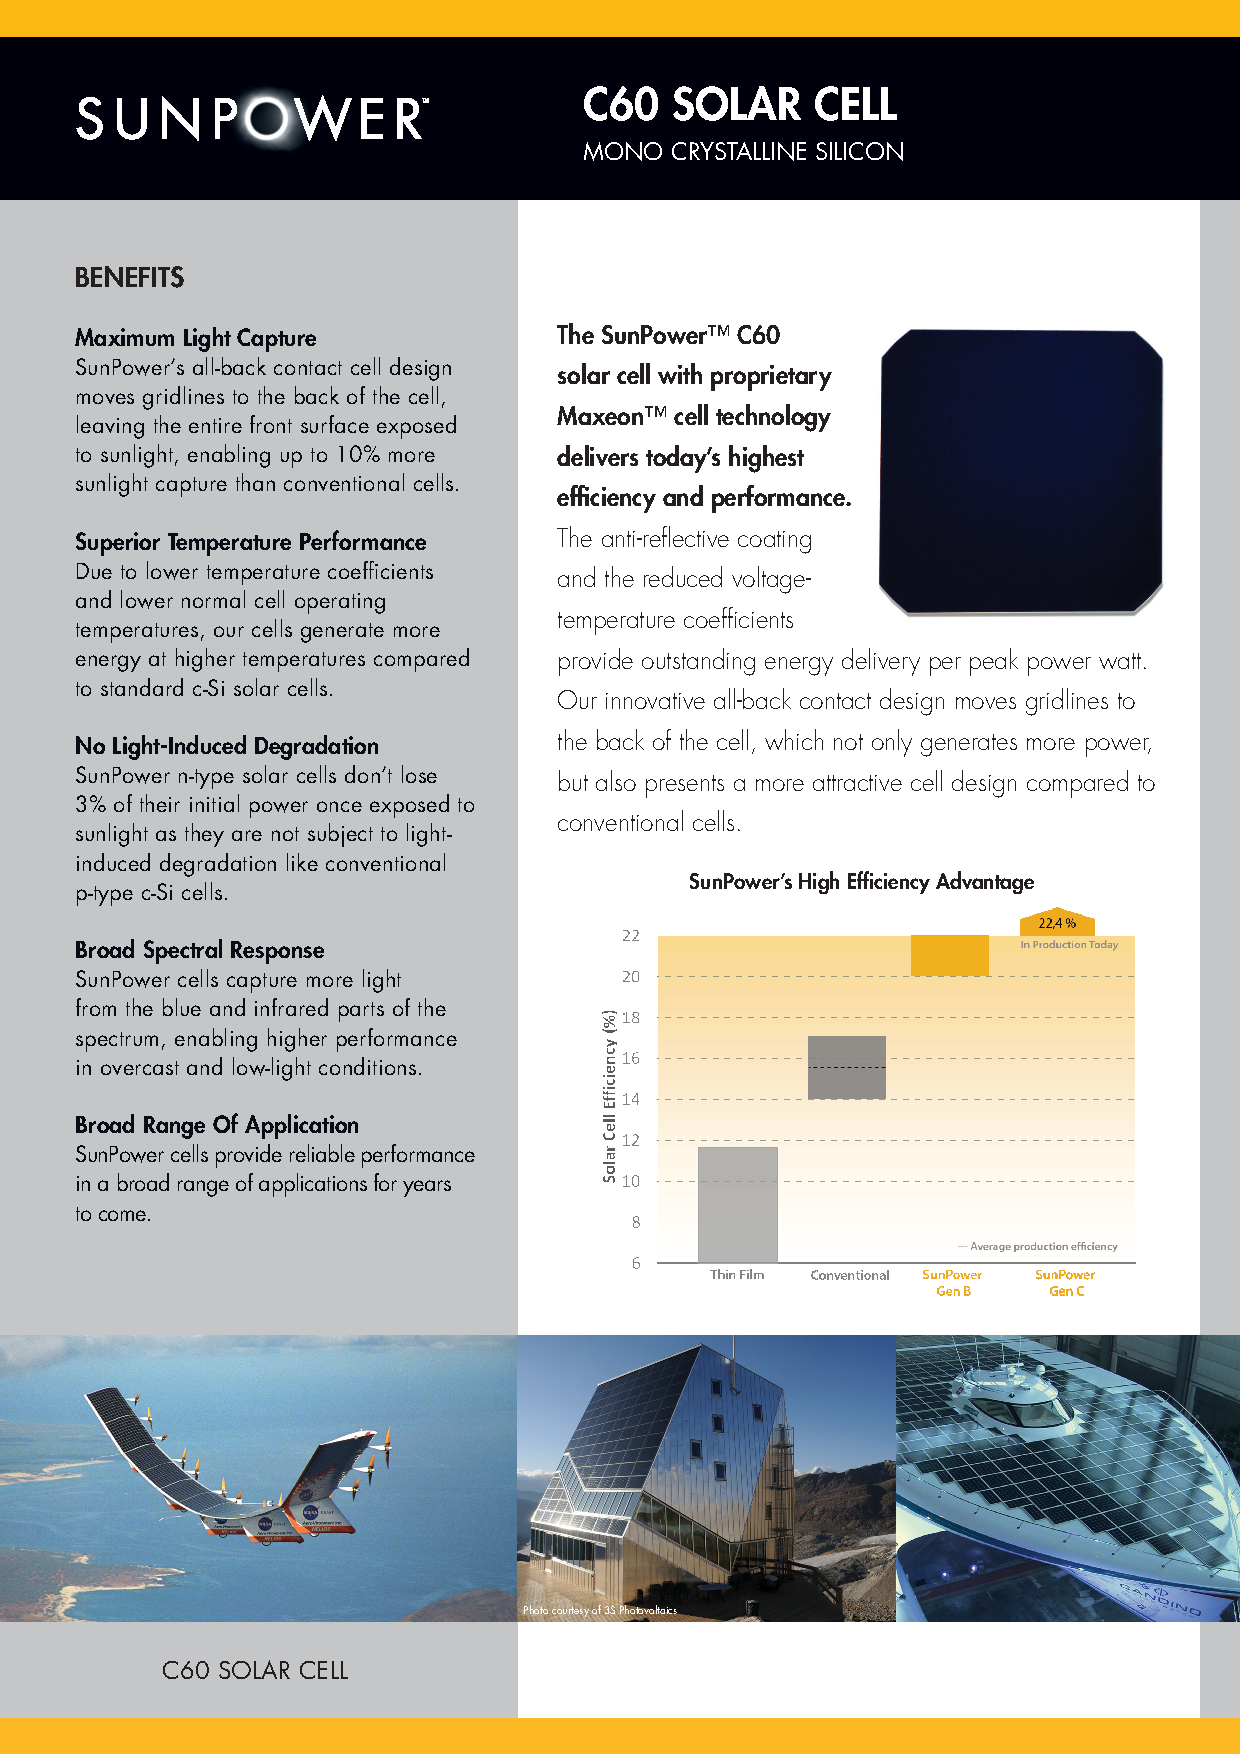
\includepdf[pages={1-2},nup=1x2,landscape=true]{Figures/SolarCell_Sunpower_C60.pdf}

 % file "Thesis_Appendix_B.tex"
%\cleardoublepage

% ----------------------------------------------------------------------
\end{document}
% ----------------------------------------------------------------------

